\section*{ANEXOS}
    %%%%%%%%%%%%%%%%%
    %   EQUAÇÕES    %
    %%%%%%%%%%%%%%%%%
    \begin{eqfloat}[h!]
        \begin{equation}
            V_{out} = \mu \cdot (V_{+} - V_{-})
            \label{eq:ganhoAmpOp}
        \end{equation}
        \caption{Fórmula para o ganho de tensão de um Amplificador Operacional.}
    \end{eqfloat}
    
    \begin{eqfloat}[h!]
        \begin{equation}
            DHT = \frac{\sqrt{(A_2)^2 + (A_3)^2 + ... + (A_4)^2}}{A_1}
            \label{eq:dht}
        \end{equation}
        \caption{Fórmula para a distorção harmônica total.}
    \end{eqfloat}
    
    
    %%%%%%%%%%%%%%%
    %   FIGURAS   %
    %%%%%%%%%%%%%%%
    \begin{figure}[h!]
        \centering
        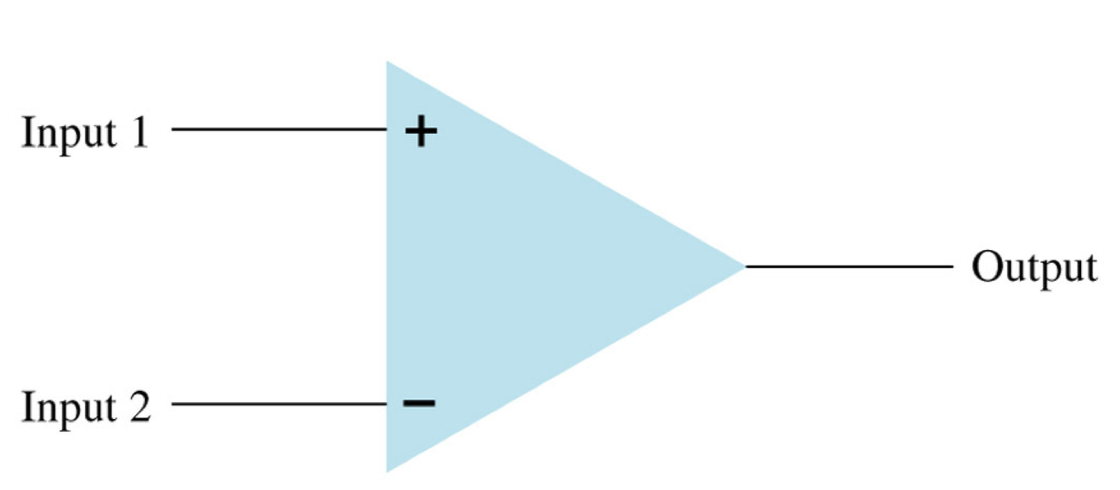
\includegraphics[height=4.5cm]{imgSource/basicAmpOp.png}
        \caption{Amp op simples.}
        \label{fig:ampOp}
    \end{figure}

    \begin{figure}[h!]
        \centering
        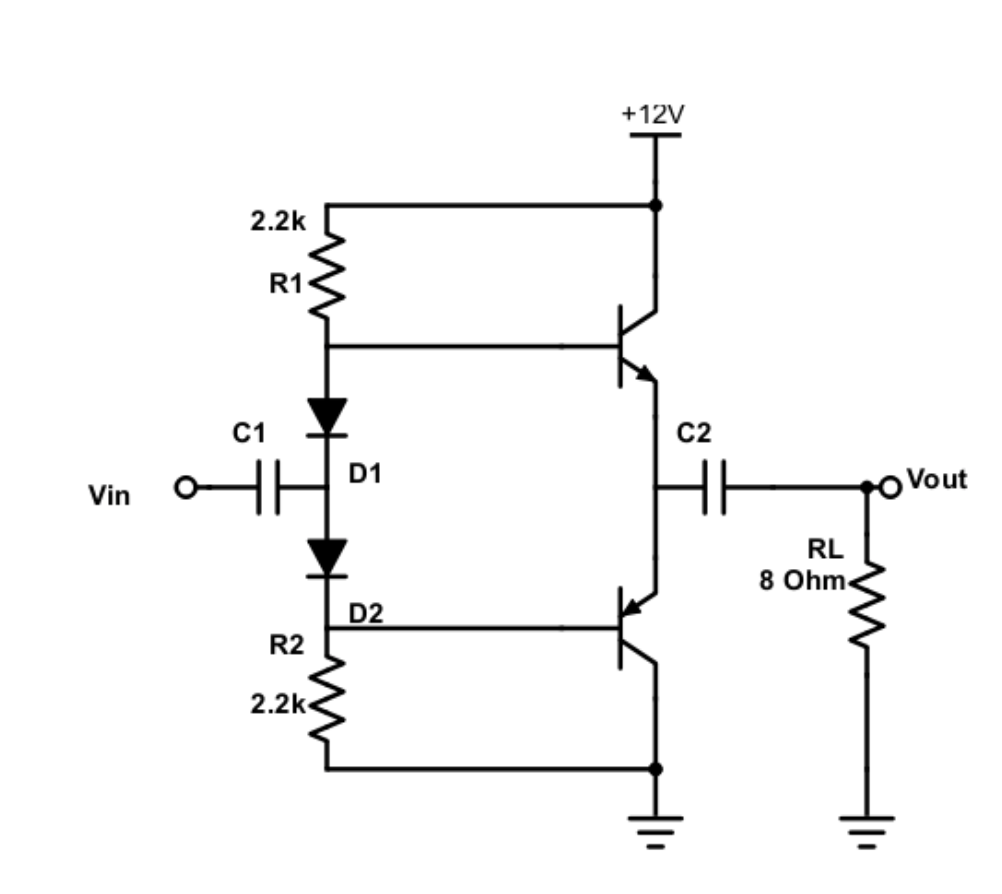
\includegraphics[height=6.5cm]{imgSource/circuits/pushPull.png}
        \caption{Circuito \emph{puh-pull} com alimentação assimétrica.}
        \label{fig:circ1}
    \end{figure}

    \begin{figure}[h!]
        \centering
        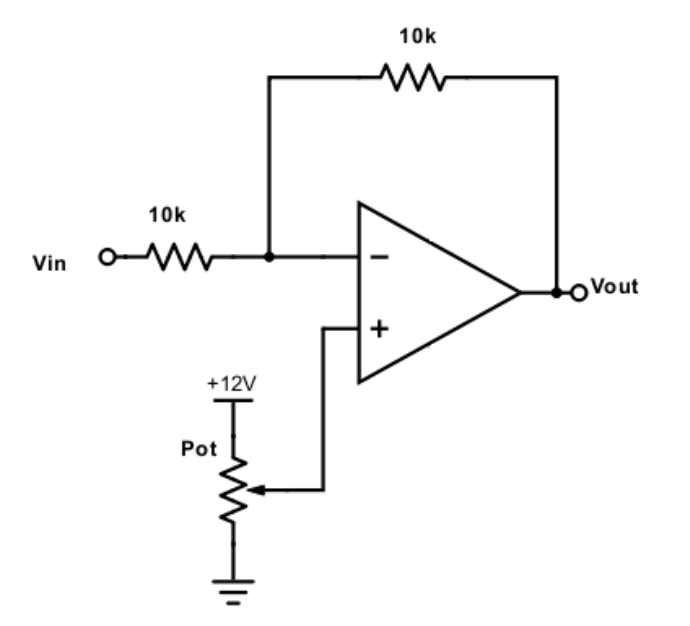
\includegraphics[height=6.5cm]{imgSource/circuits/ampOp1.png}
        \caption{Circuito com um \emph{Amp-op}.}
        \label{fig:circ2}
    \end{figure}
    
    \begin{figure}[h!]
        \centering
        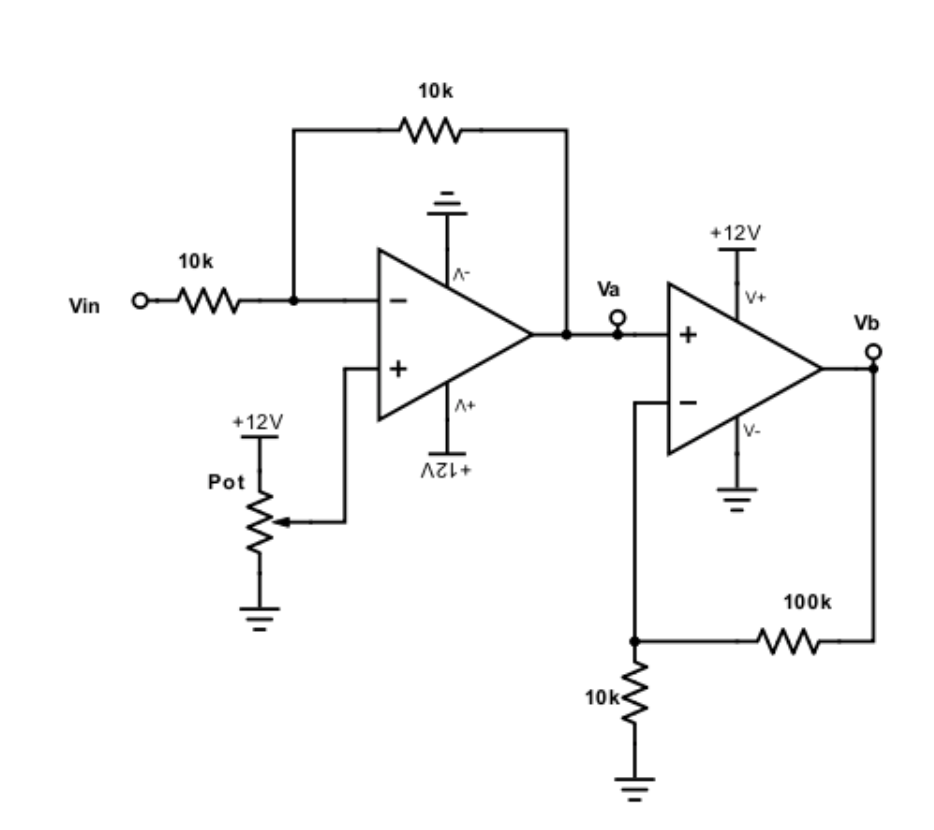
\includegraphics[height=6.5cm]{imgSource/circuits/ampOp2.png}
        \caption{Circuito com dois \emph{Amp-ops}.}
        \label{fig:circ3}
    \end{figure}
    
    \begin{figure}[h!]
        \centering
        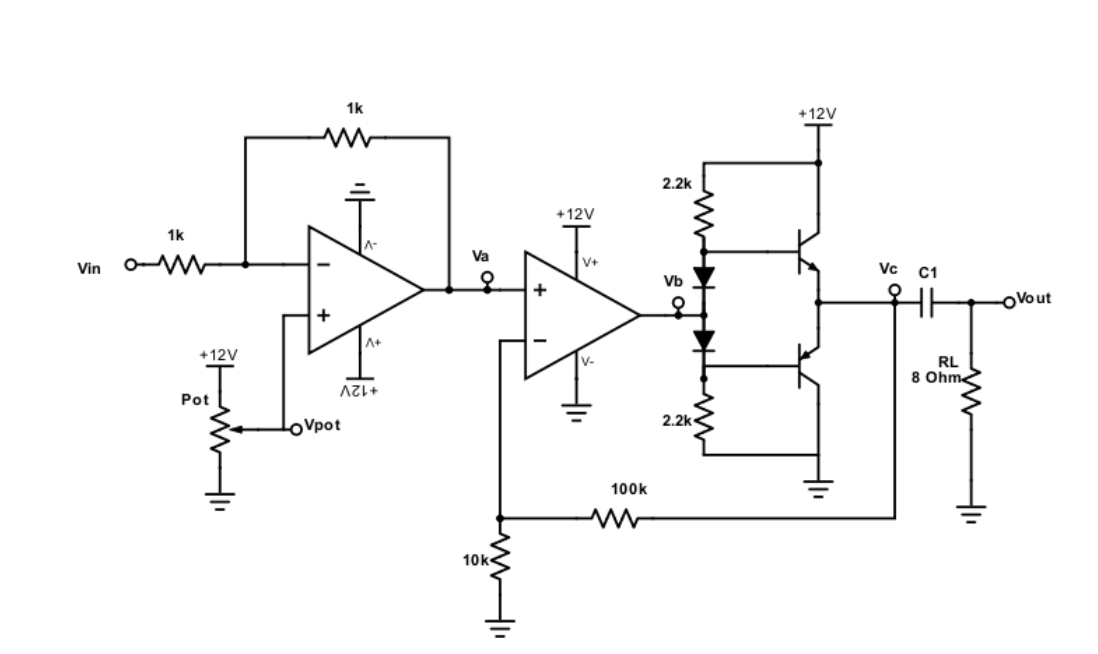
\includegraphics[height=6.5cm]{imgSource/circuits/ampOpPush.png}
        \caption{Circuito \emph{puh-pull} com alimentação não-simétrica e realimentação.}
        \label{fig:circ4}
    \end{figure}
    
    \begin{figure}[h!]
        \centering
        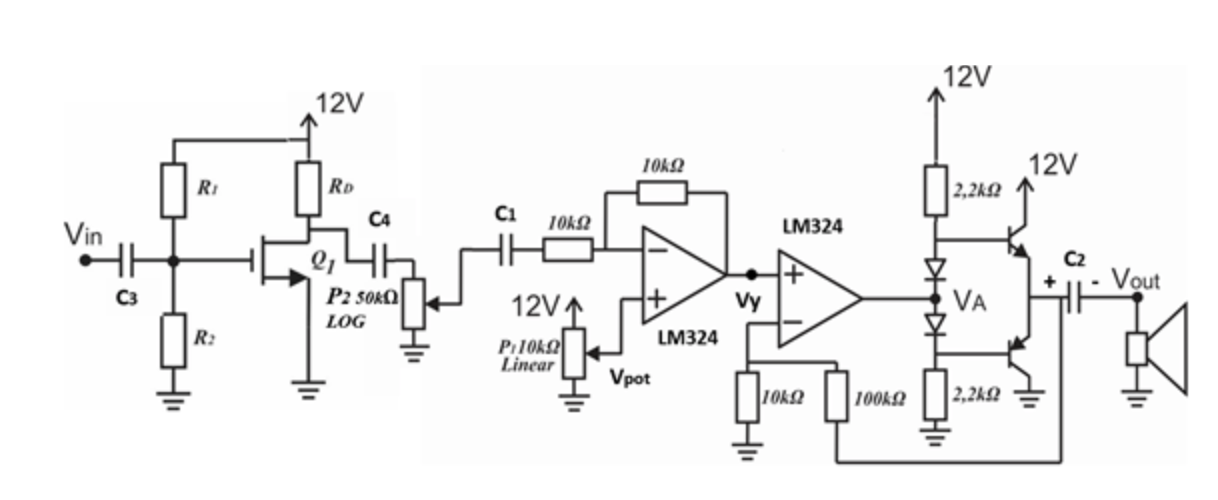
\includegraphics[height=6.5cm]{imgSource/circuits/monstro.png}
        \caption{Circuito completo, com estágio de ganho e estágio de potência realimentado.}
        \label{fig:circ5}
    \end{figure}
    
    \begin{figure}[h!]
        \centering
        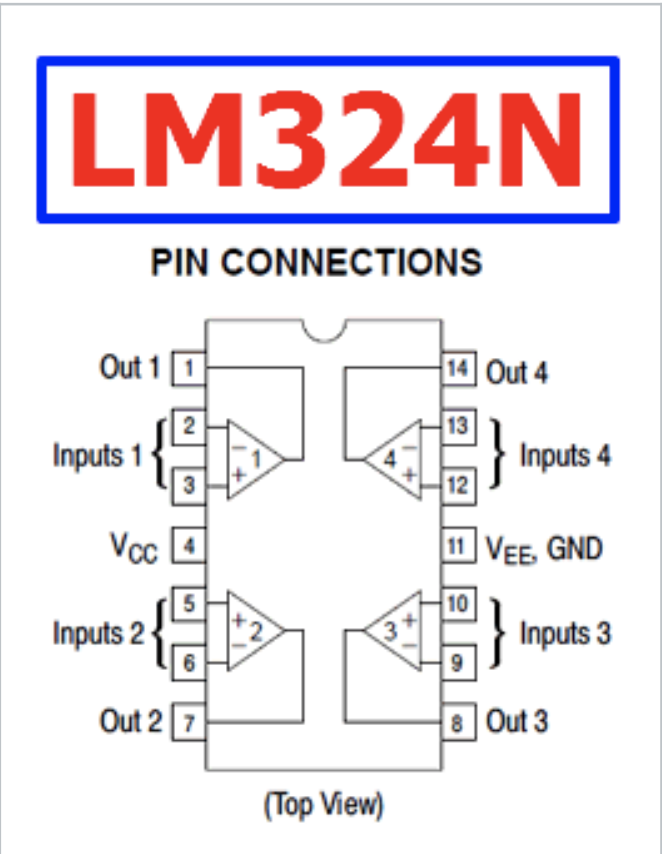
\includegraphics[height=6.5cm]{imgSource/ampOpPorts.png}
        \caption{Discriminação do circuito interno do amplificador operacional LM324.}
        \label{fig:circAmpOp}
    \end{figure}

    \begin{figure}[h!]
        \centering
        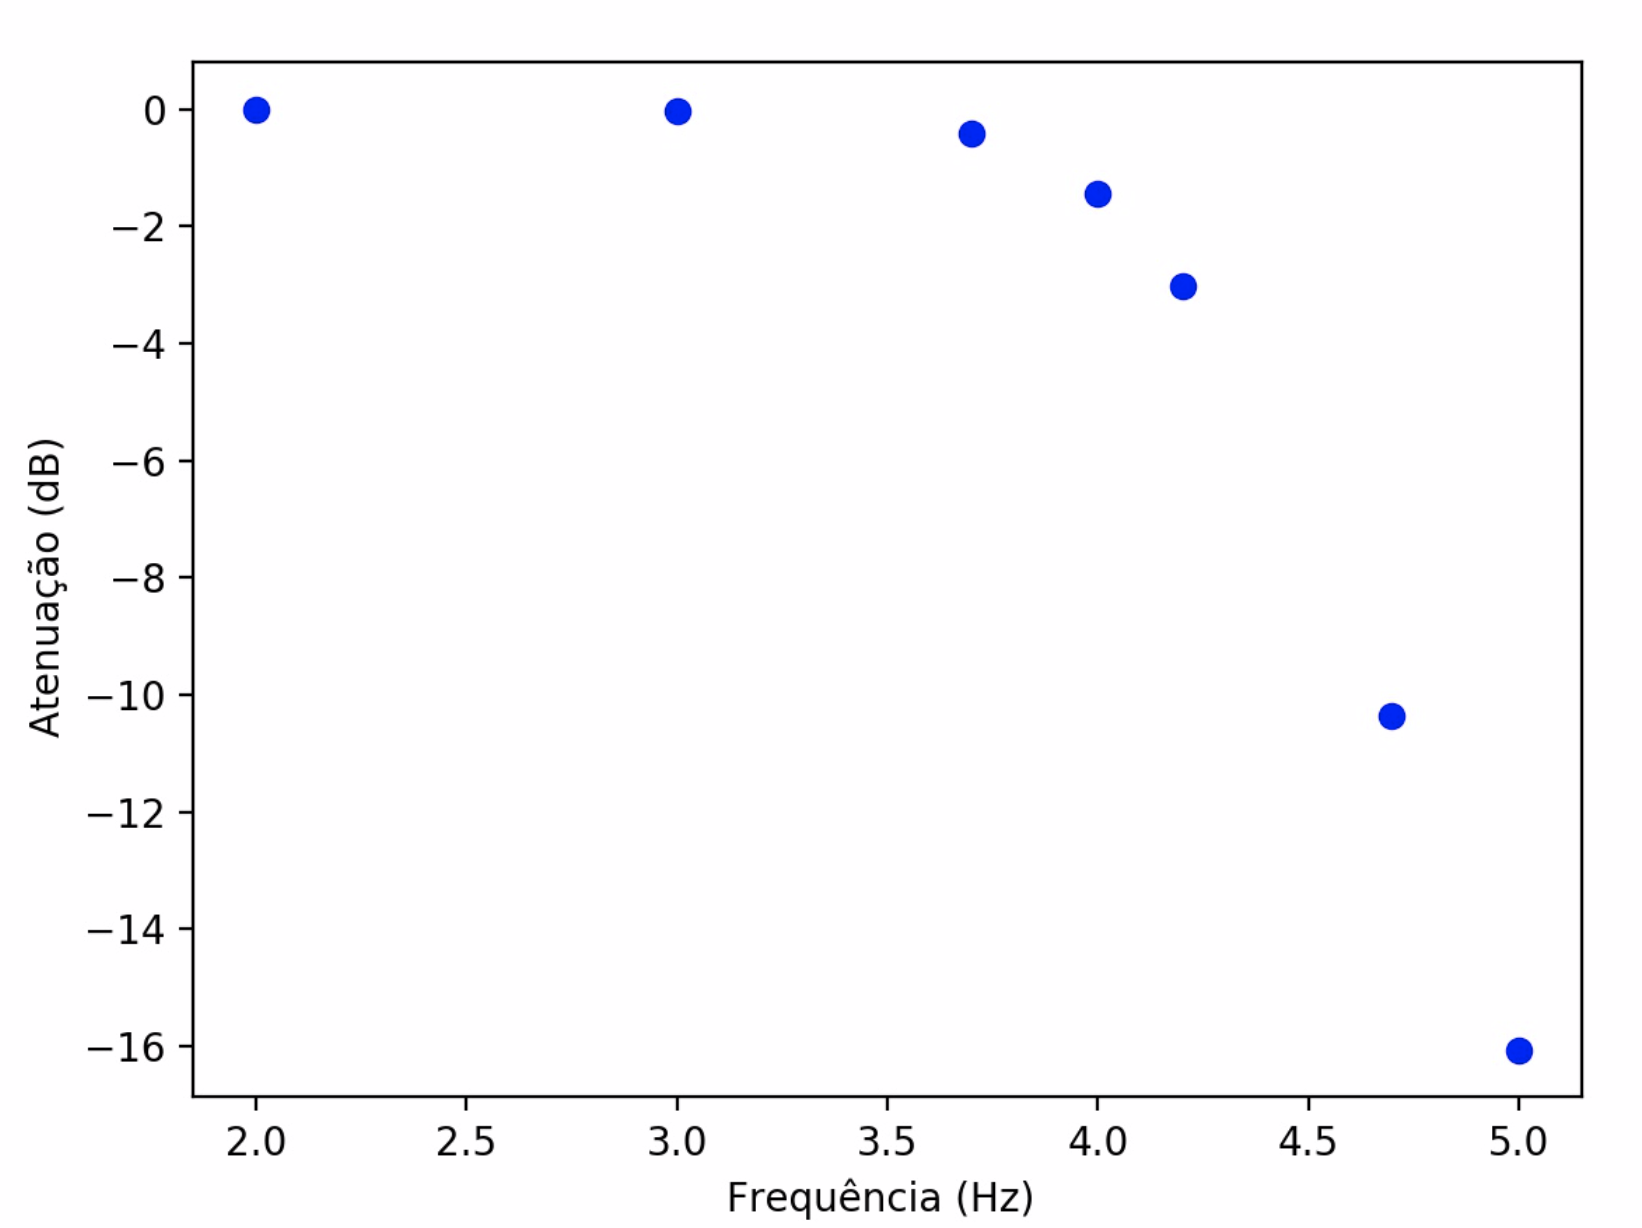
\includegraphics[height=6.5cm]{imgSource/charts/passabaixa.png}
        \caption{Digrama de bode de um filtro passa baixa.}
        \label{fig:passaBaixa}
    \end{figure}
   
    \begin{figure}[h!]
        \centering
        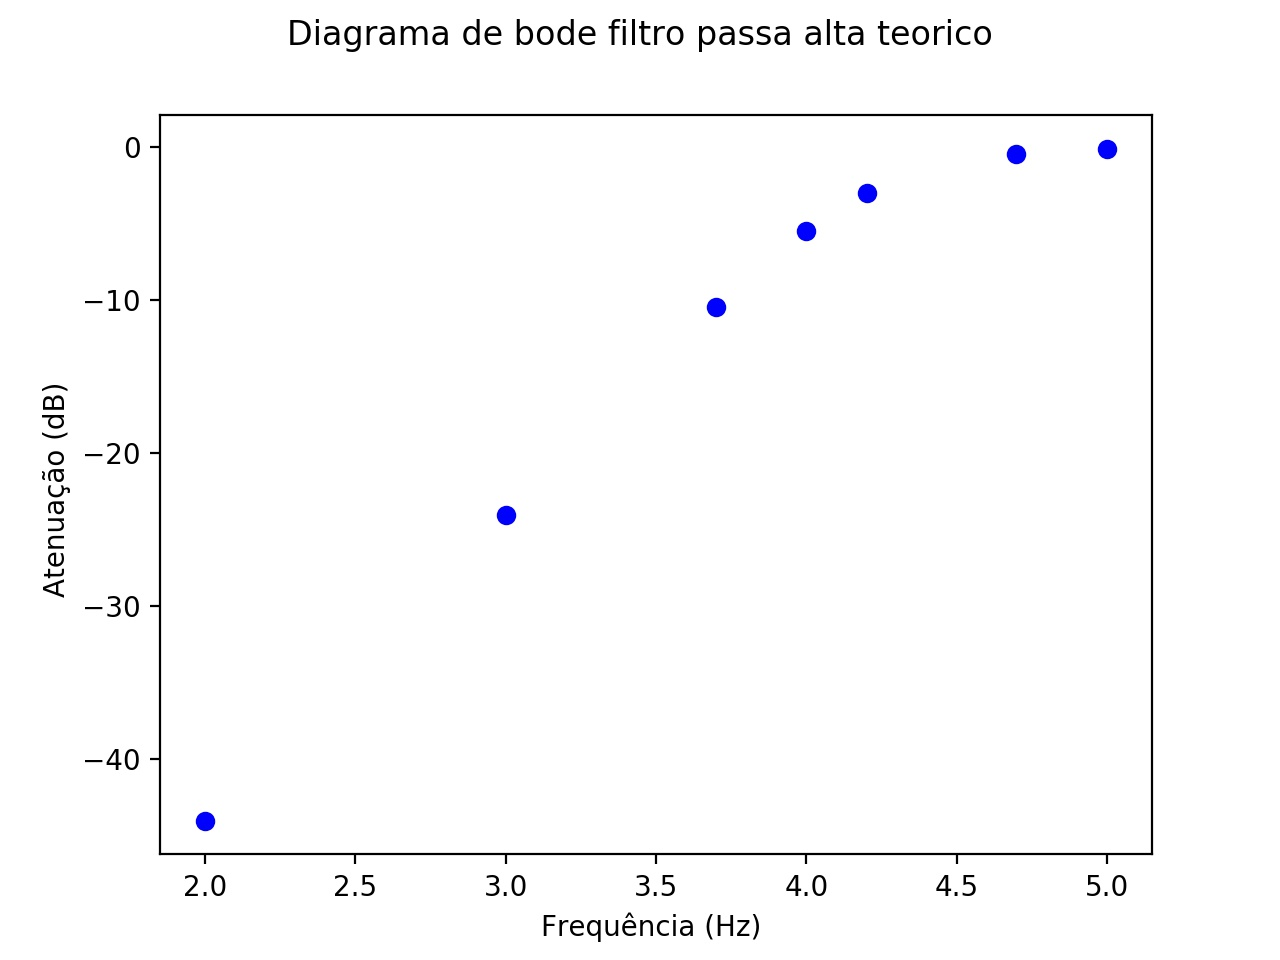
\includegraphics[height=6.5cm]{imgSource/charts/passaalta.jpg}
        \caption{Digrama de bode de um filtro passa alta.}
        \label{fig:passaAlta}
    \end{figure}

   \begin{figure}[h!]
        \centering
        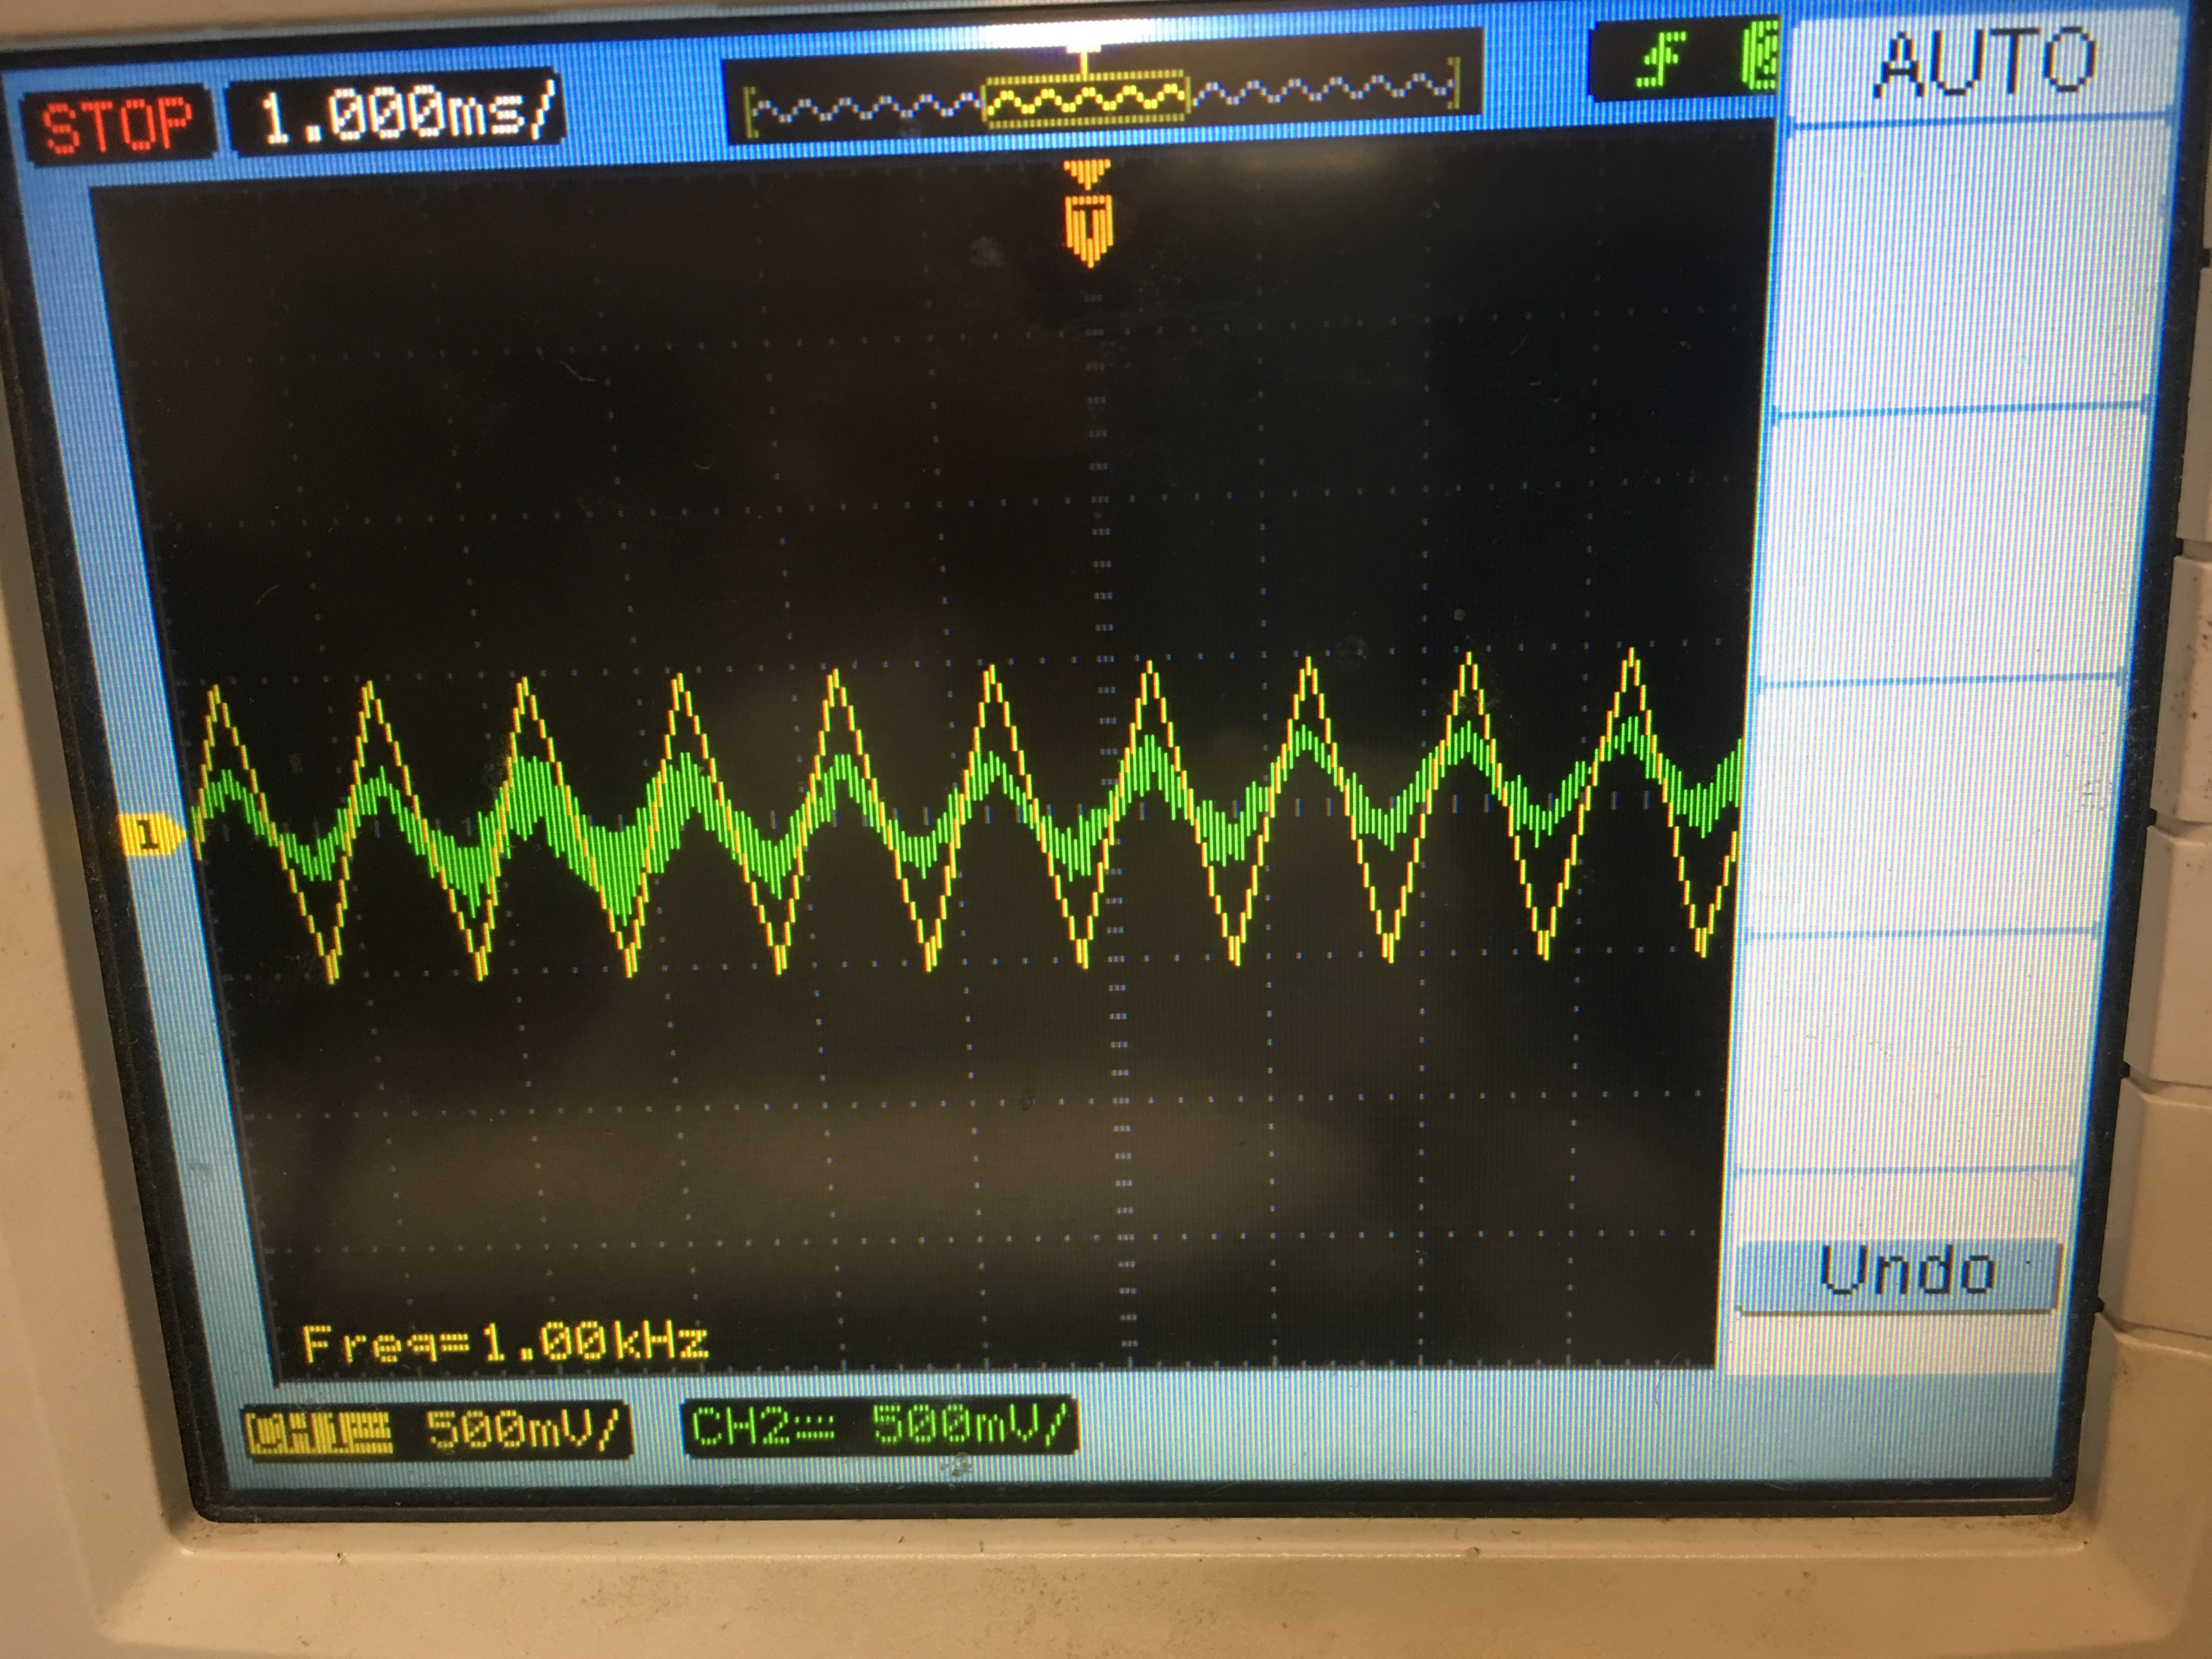
\includegraphics[height=6.5cm]{imgSource/oscilloscope/foto0.jpg}
        \caption{Sinal de saída do circuito push-pull a 500mV e 1KHz.}
        \label{fig:foto1}
    \end{figure}
    
    \begin{figure}[h!]
        \centering
        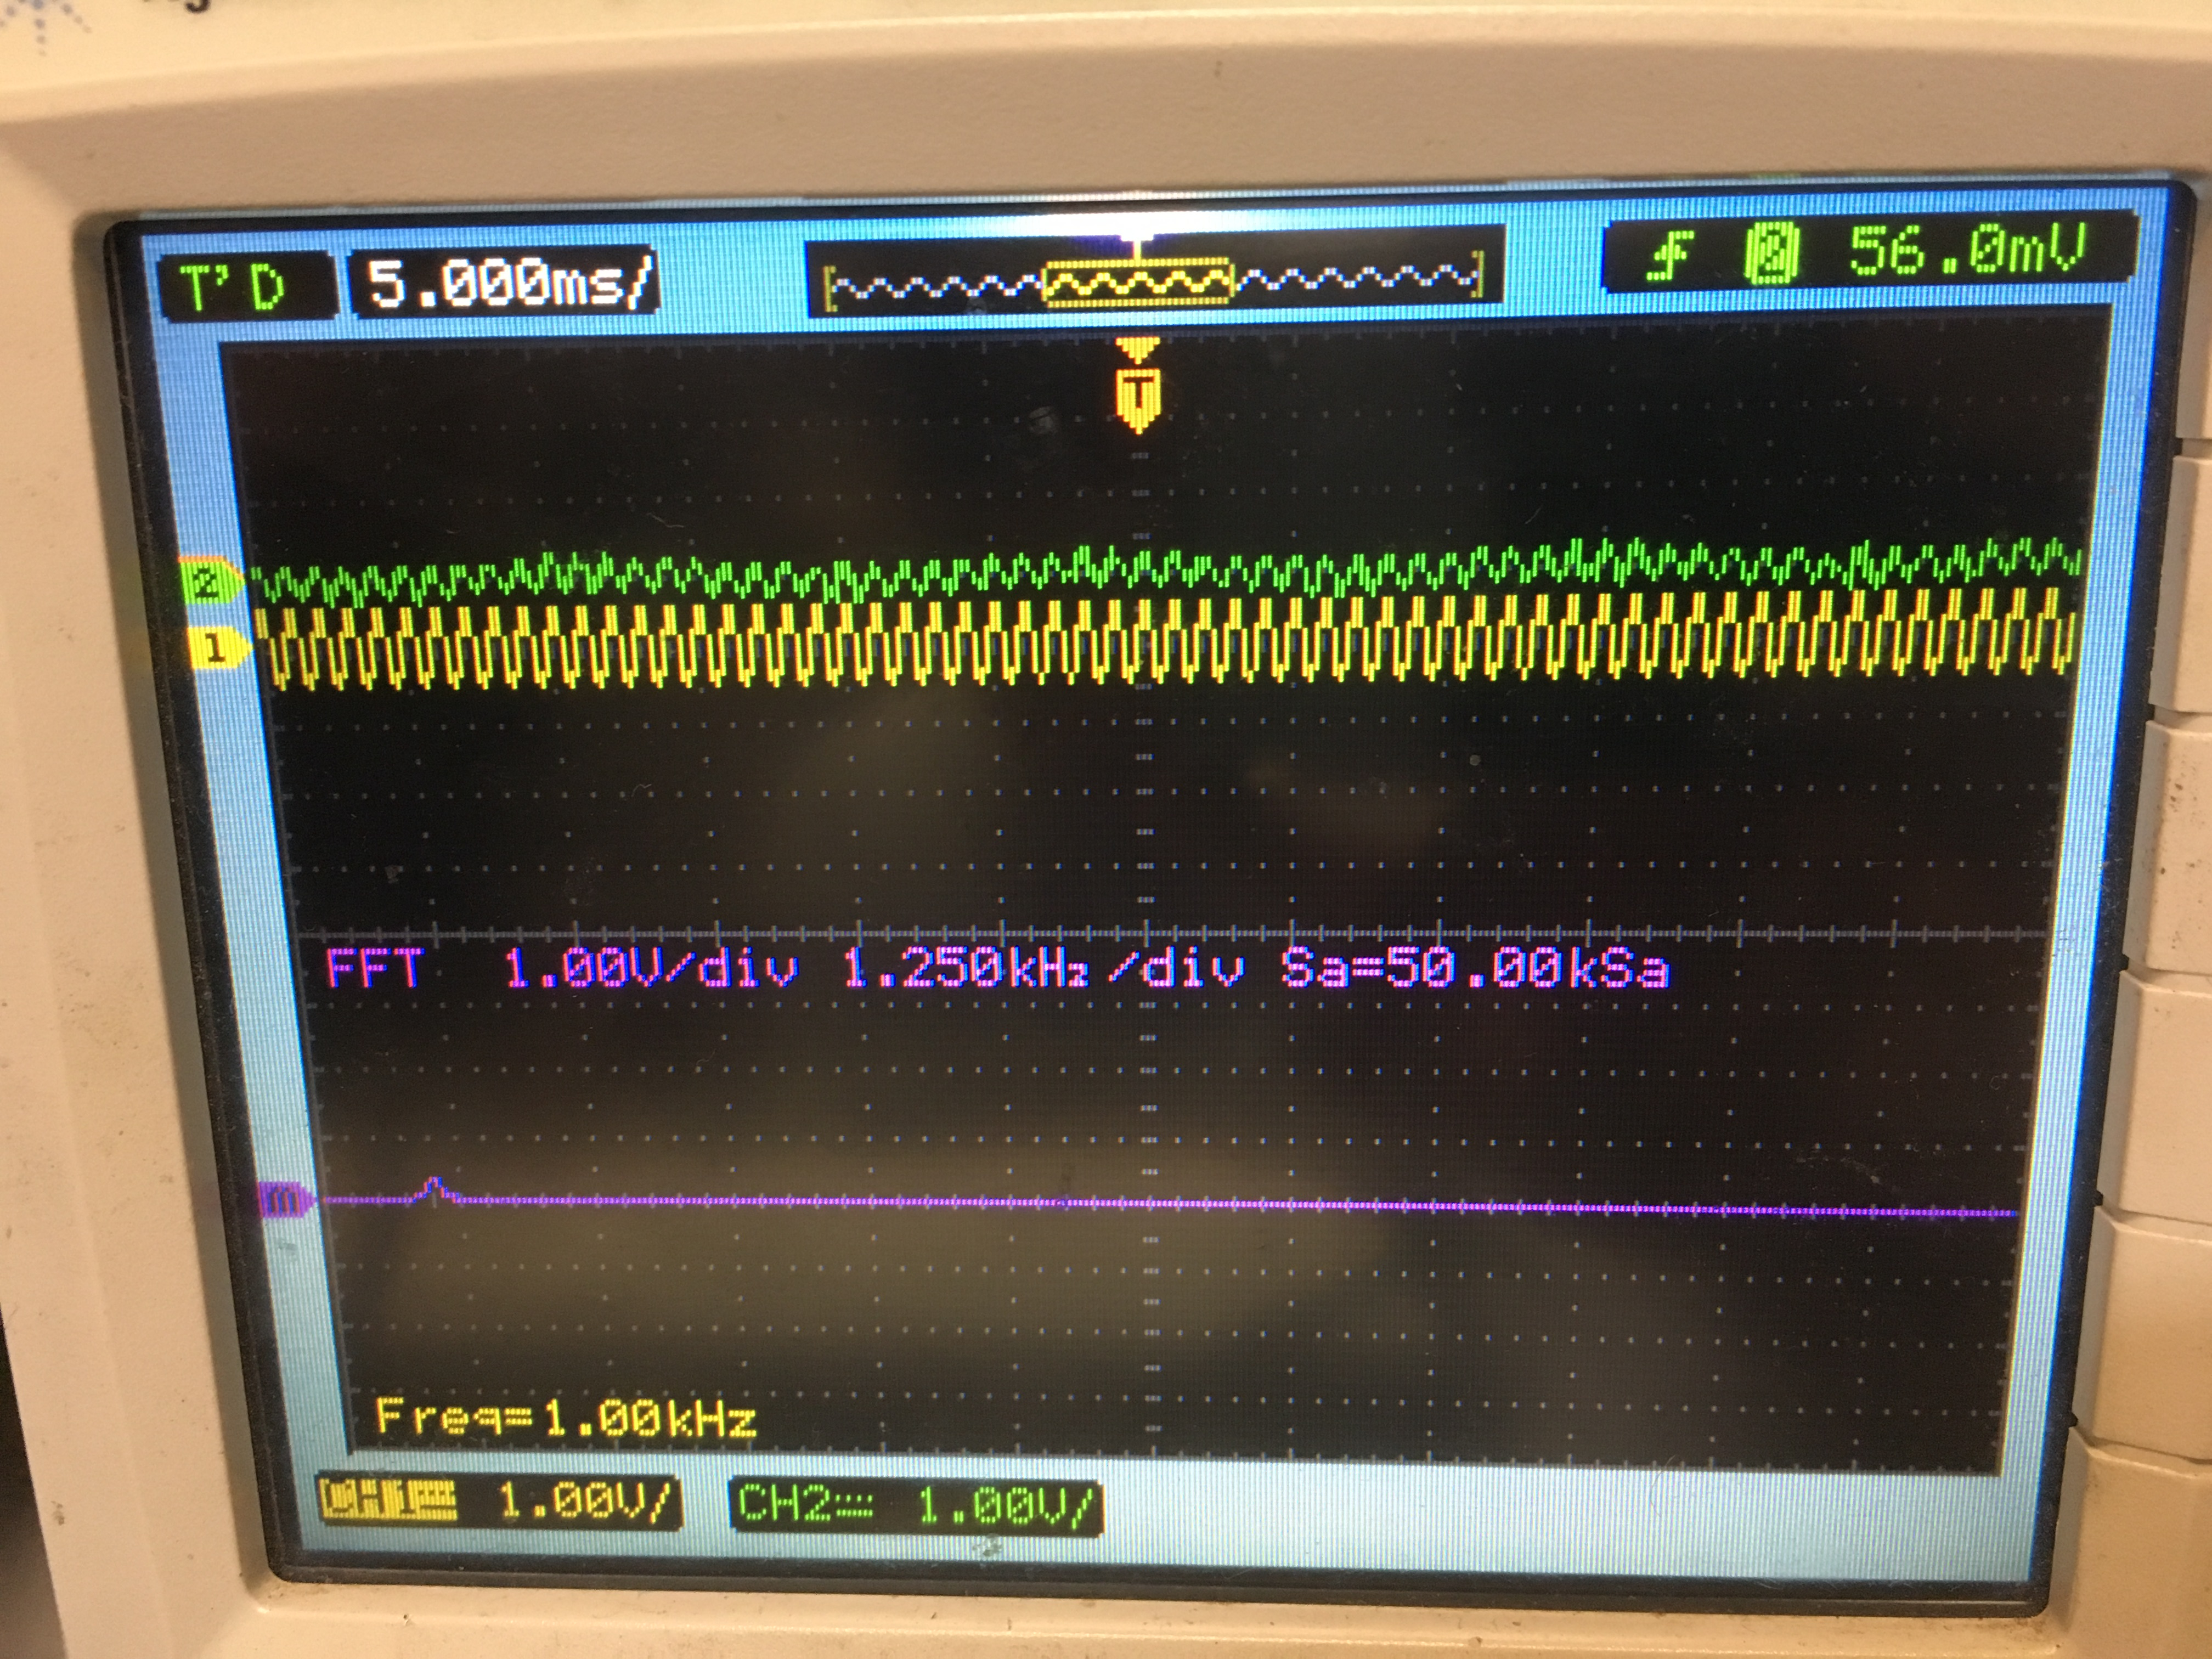
\includegraphics[height=6.5cm]{imgSource/oscilloscope/foto1.jpg}
        \caption{Espectro da onda de saída.}
        \label{fig:foto2}
    \end{figure}
   
    \begin{figure}[h!]
        \centering
        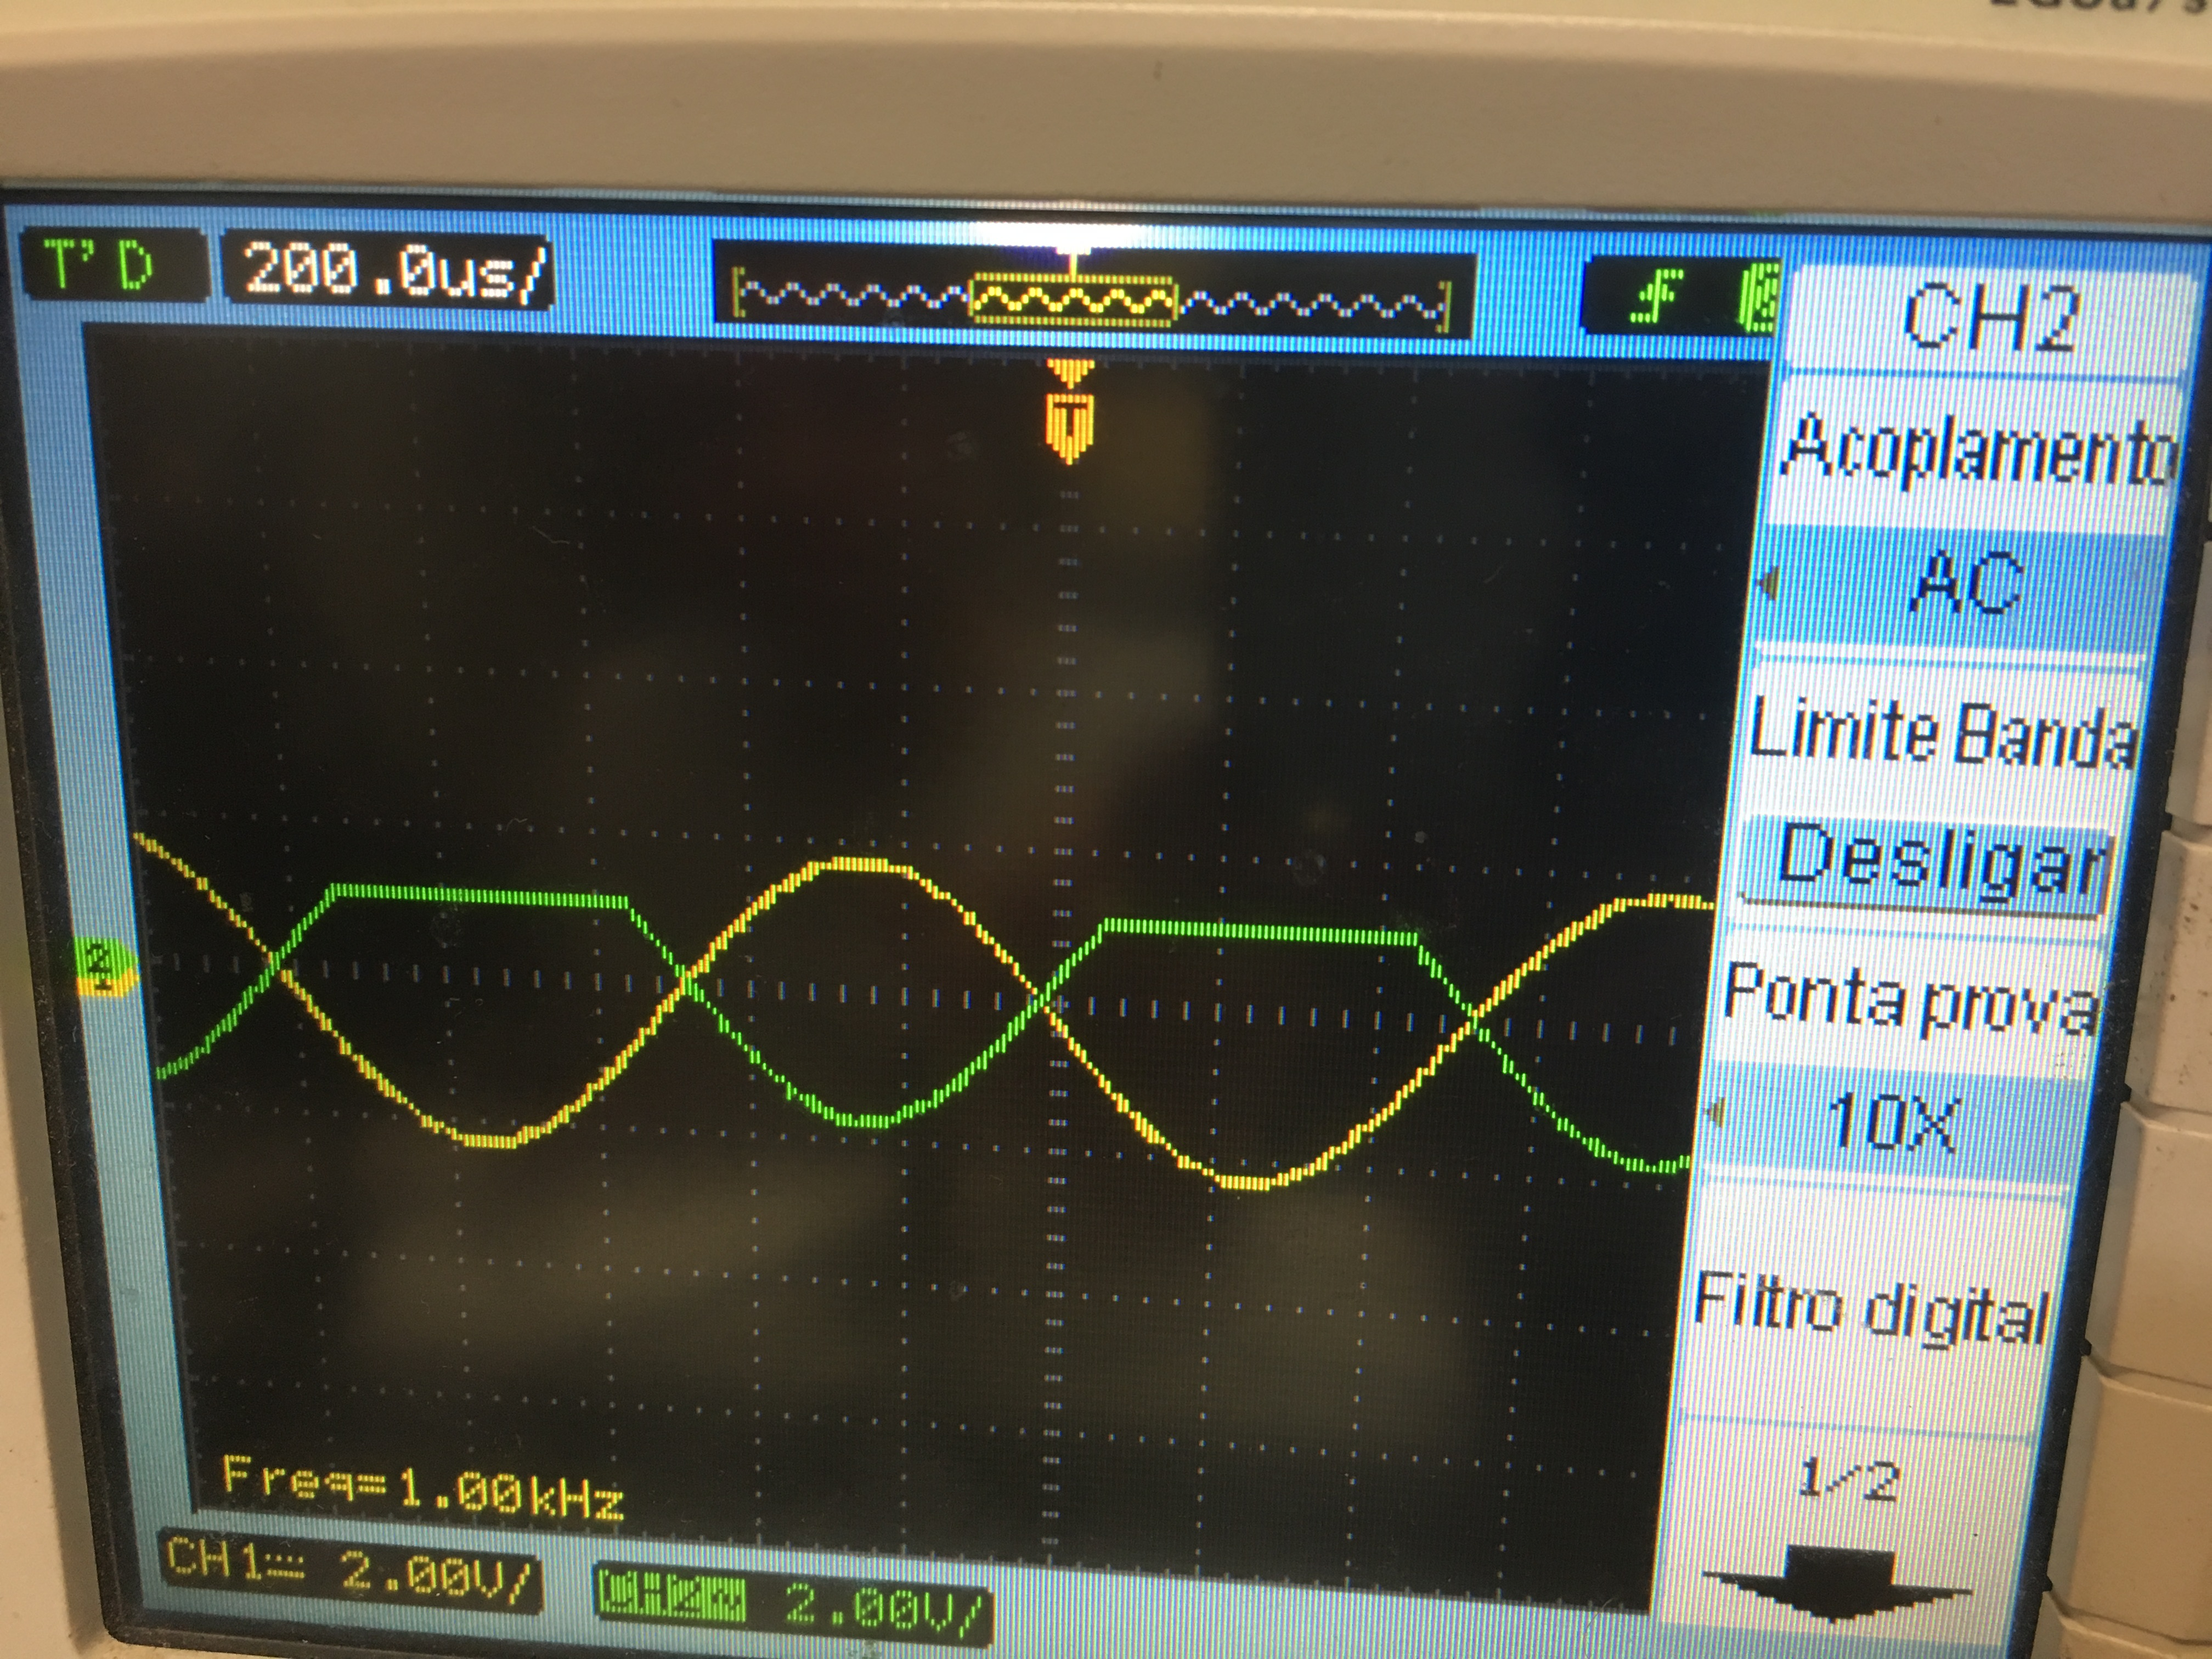
\includegraphics[height=6.5cm]{imgSource/oscilloscope/foto2.jpg}
        \caption{Sinal de saída do circuito montado a partir do amplificador operacional.}
        \label{fig:foto3}
    \end{figure}

    \begin{figure}[h!]
        \centering
        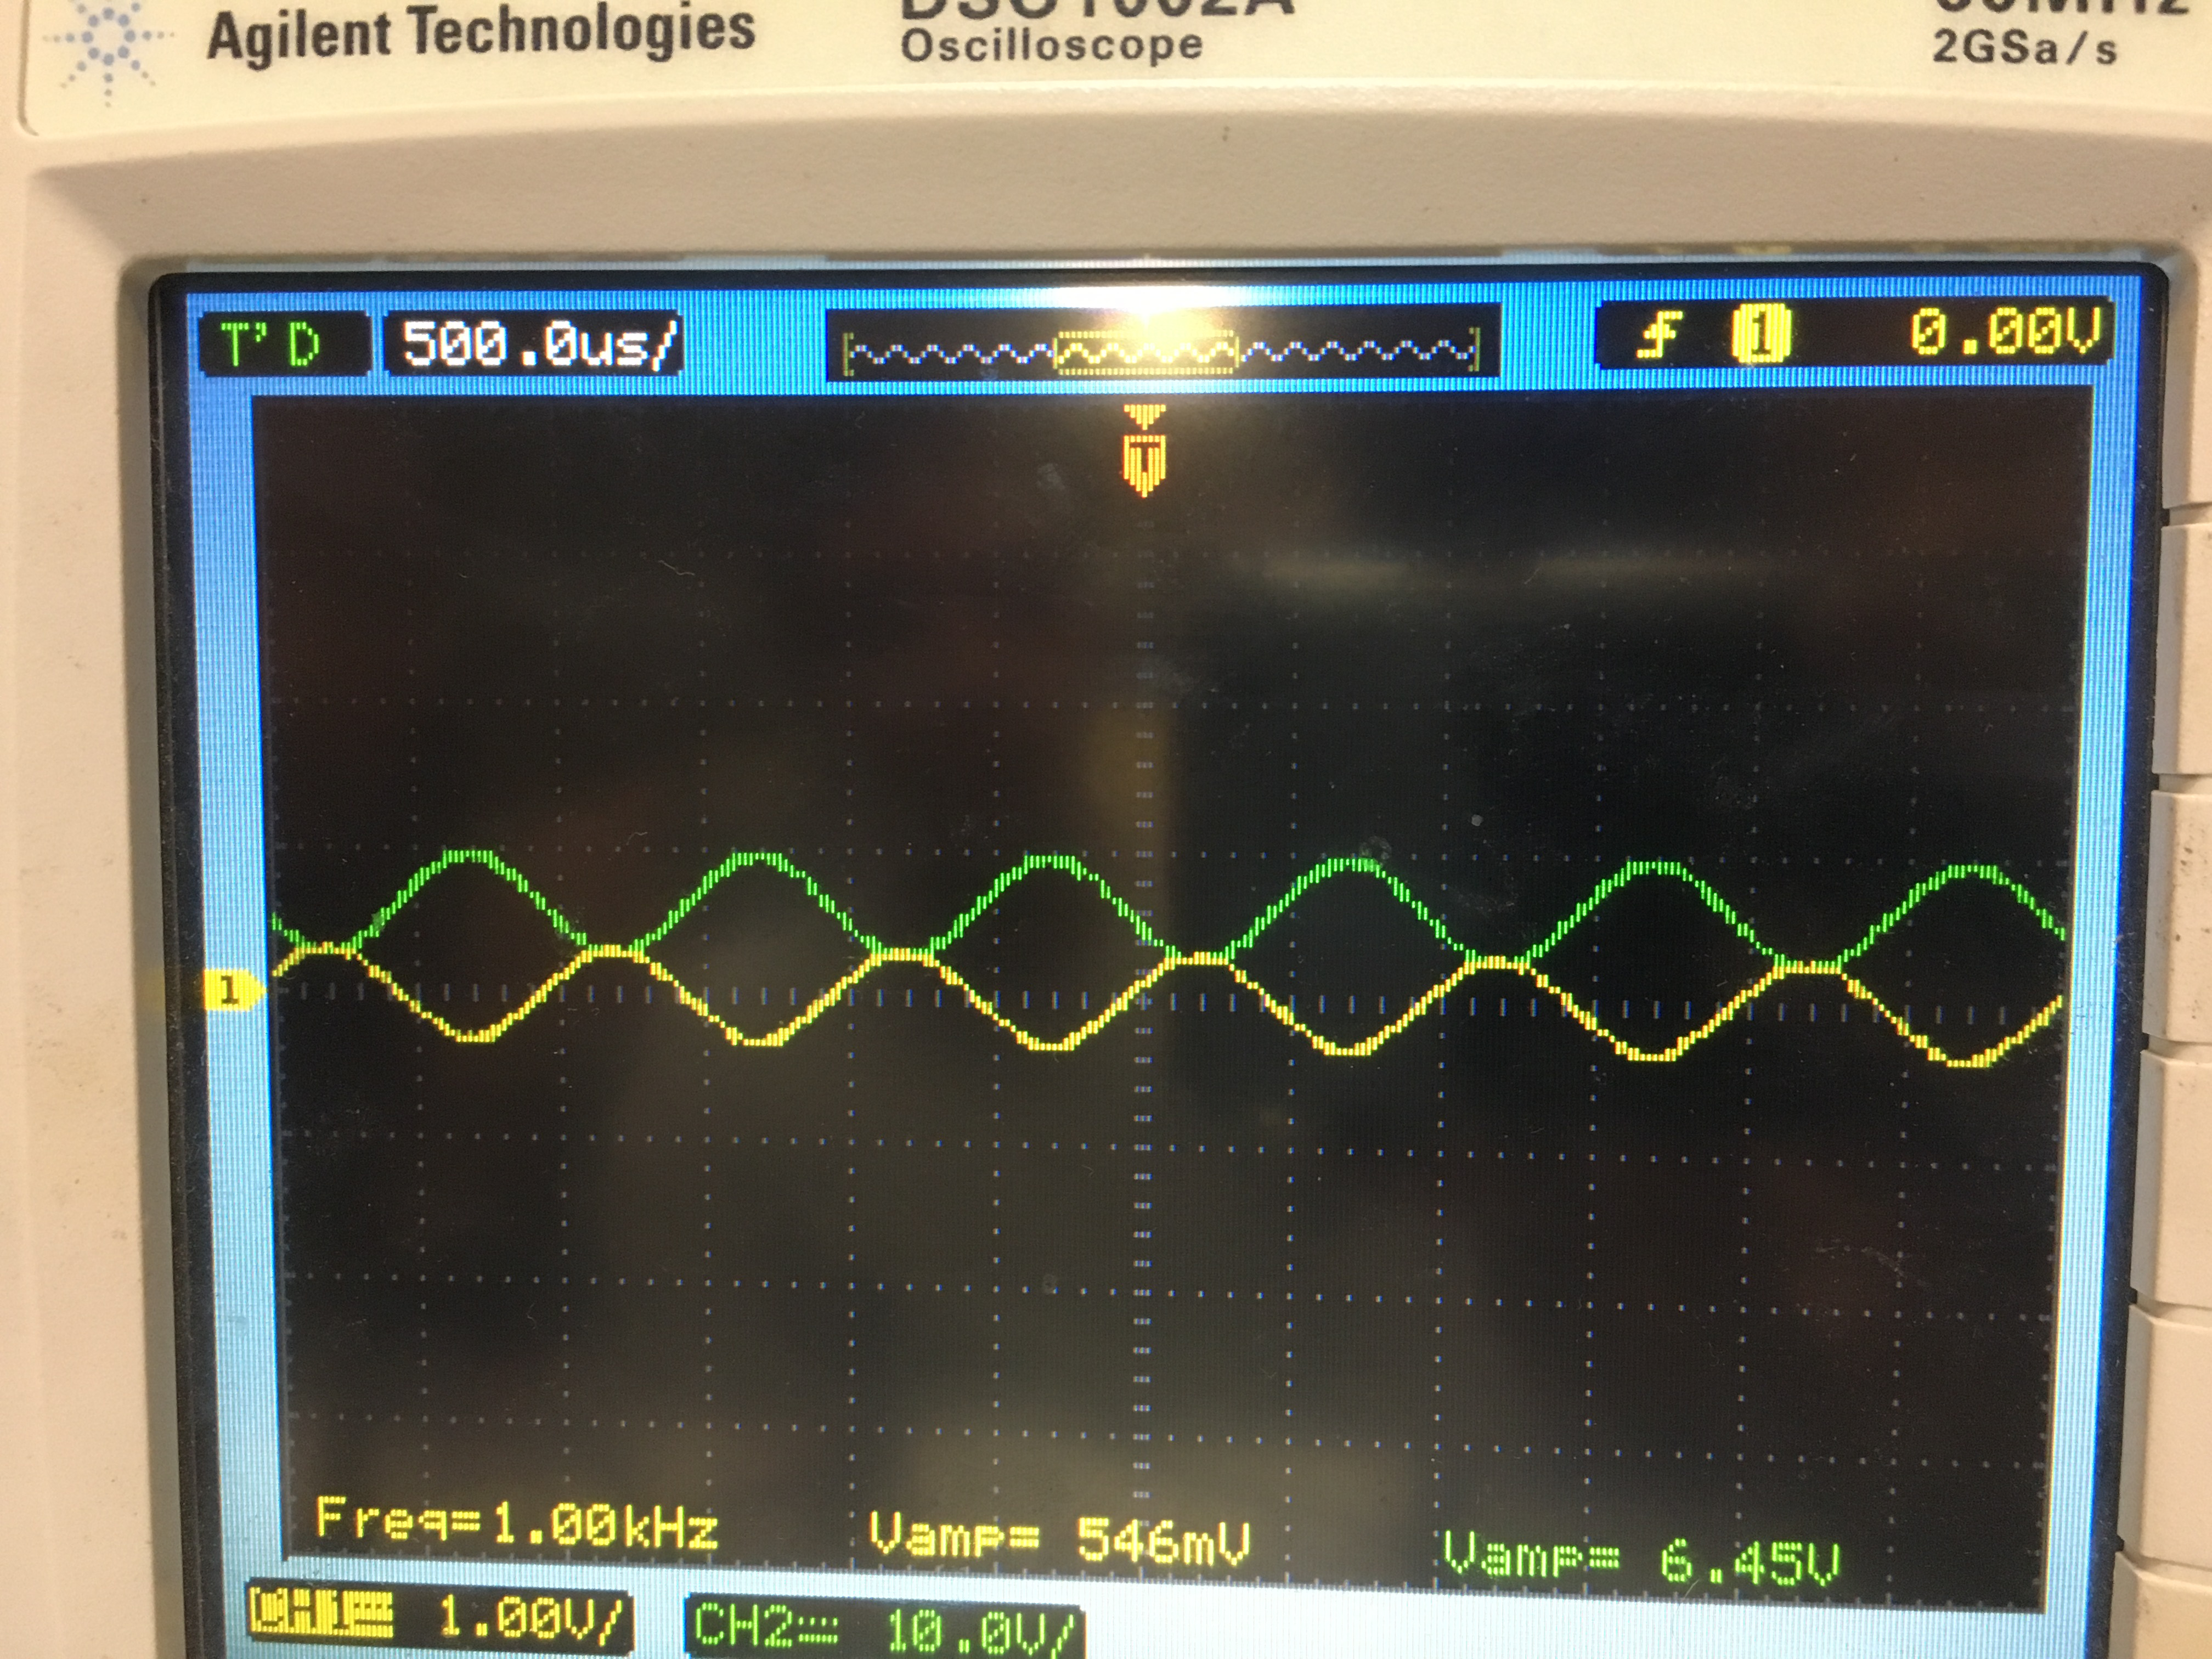
\includegraphics[height=6.5cm]{imgSource/oscilloscope/foto5.jpg}
        \caption{Sinal de saída com máxima excursão.}
        \label{fig:foto7}
    \end{figure}

    \begin{figure}[h!]
        \centering
        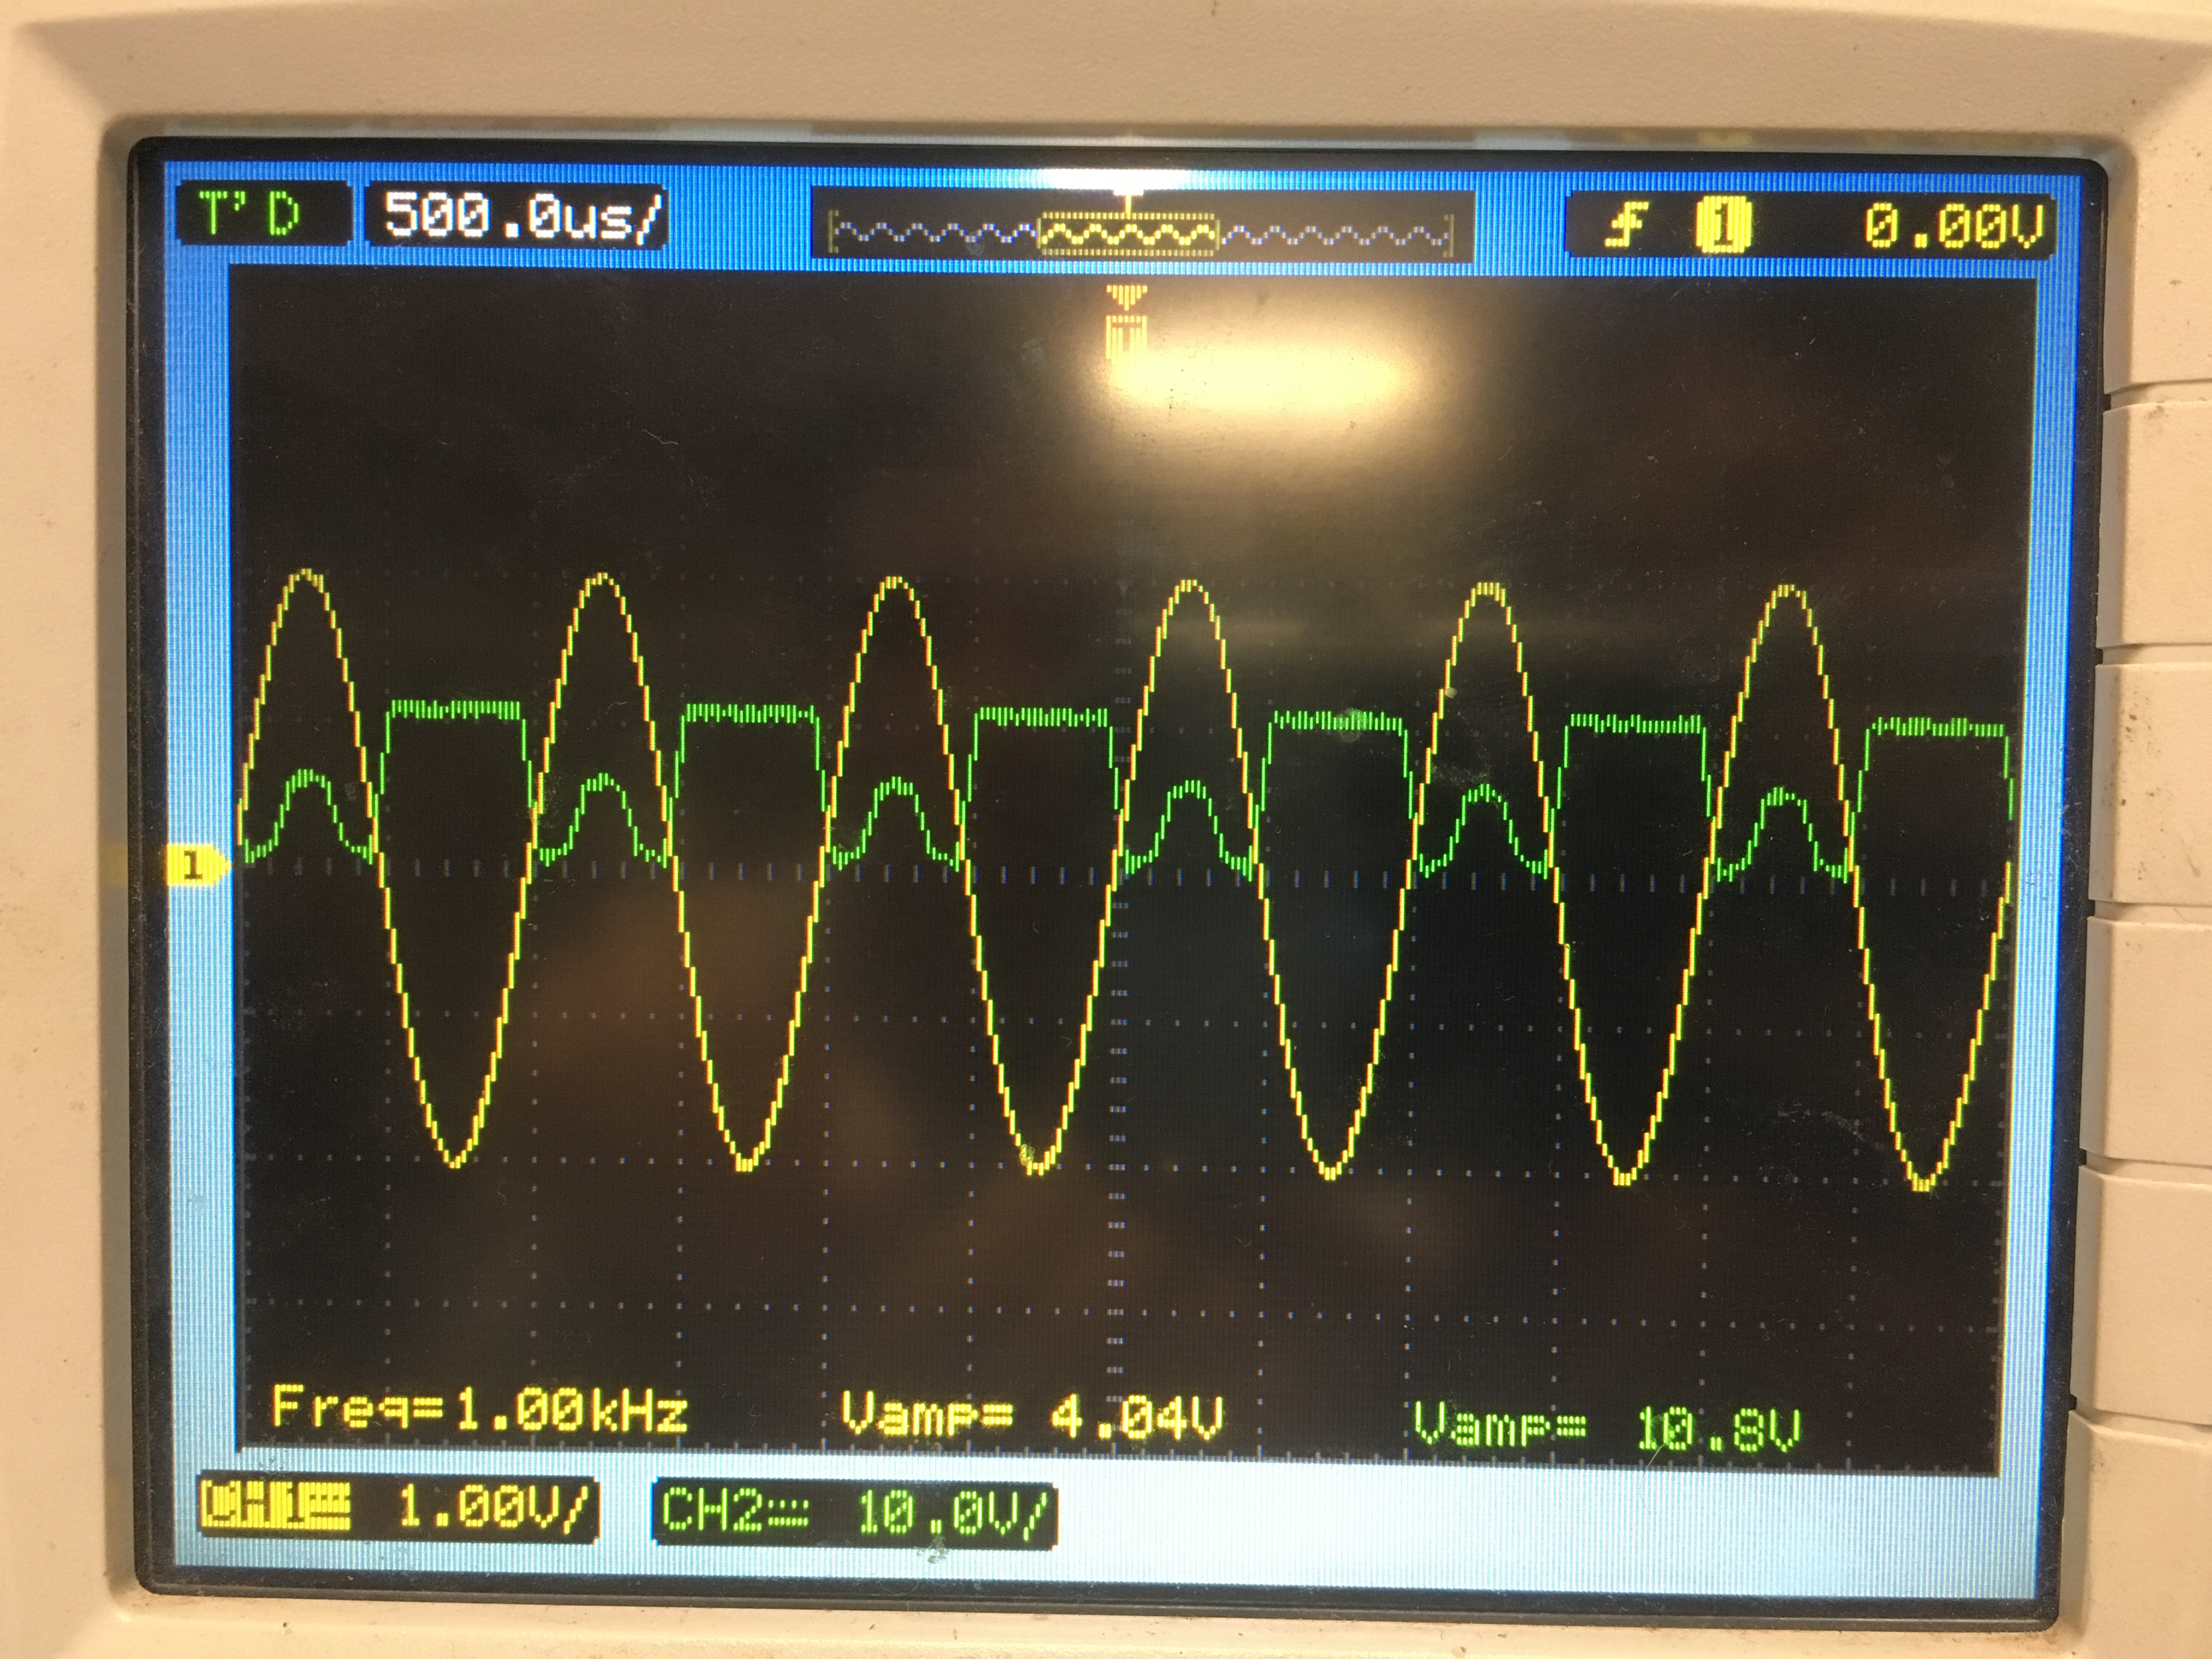
\includegraphics[height=6.5cm]{imgSource/oscilloscope/foto6.jpg}
        \caption{Sinal de saída saturado superiormente para o circuito montado com dois amplificadores operacionais acoplados.}
        \label{fig:foto6}
    \end{figure}

    \begin{figure}[h!]
        \centering
        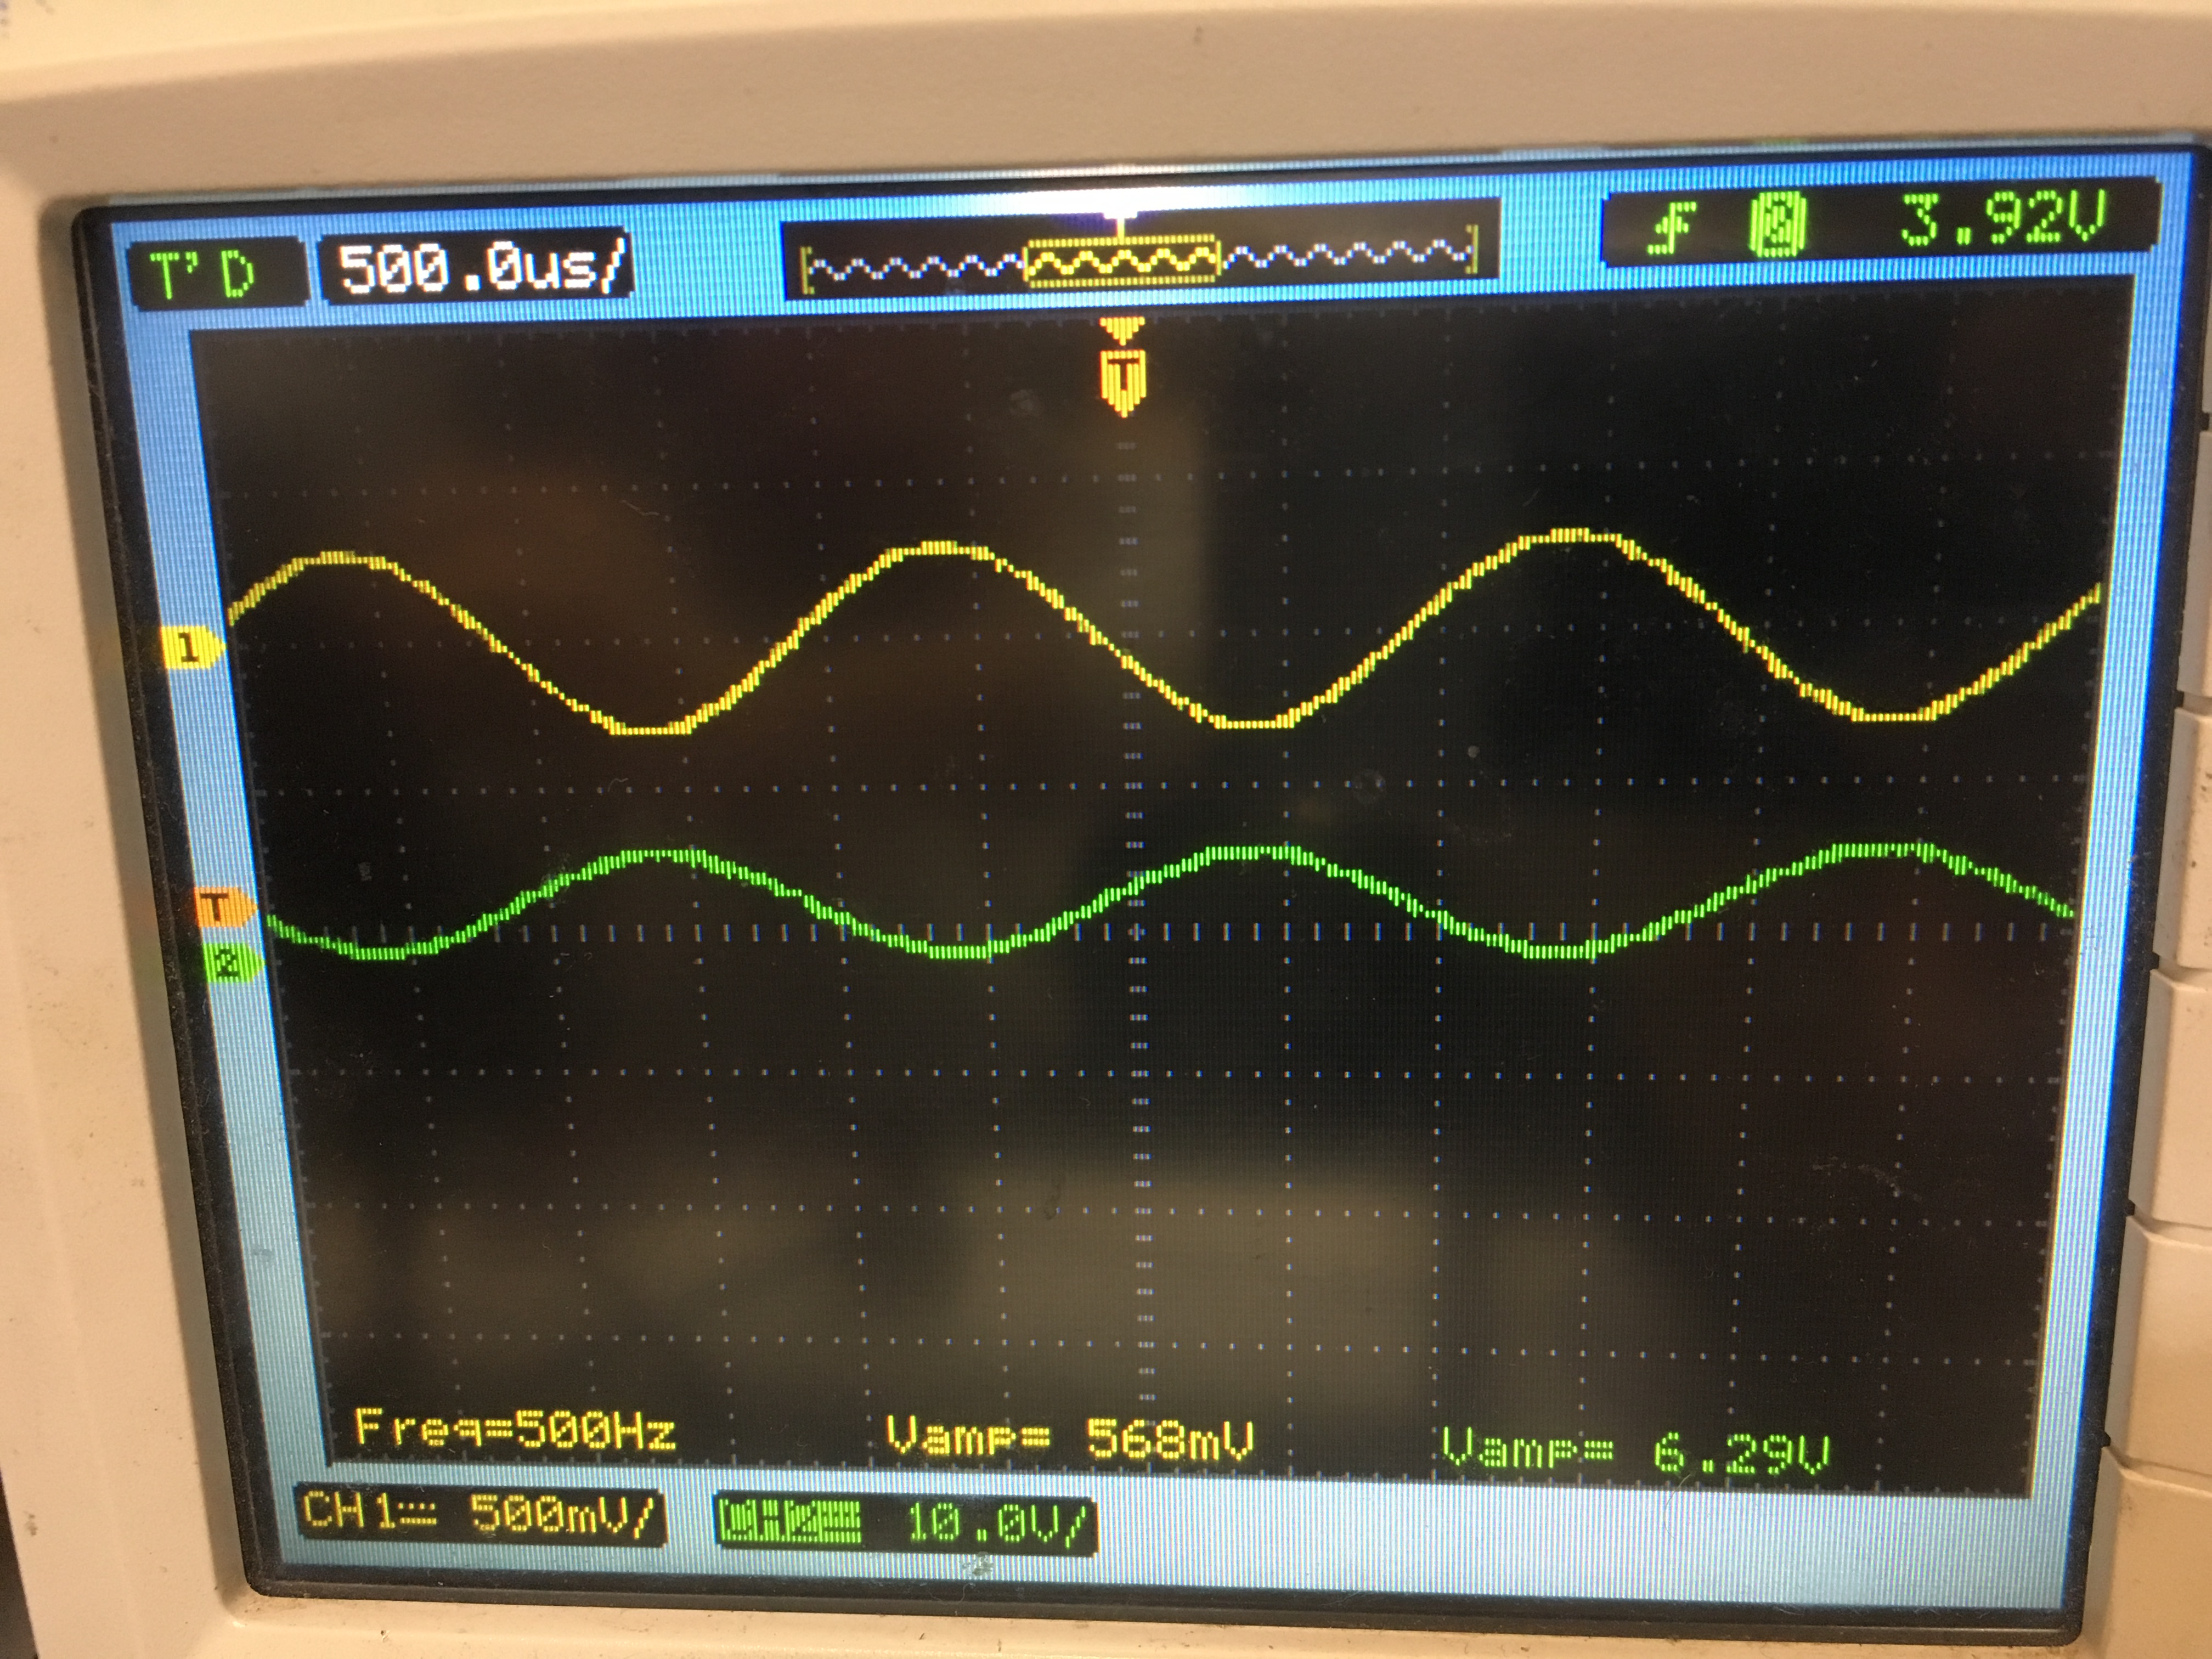
\includegraphics[height=6.5cm]{imgSource/oscilloscope/foto8.jpg}
        \caption{Sinal de saída para uma entrada com frequência de 500Hz.}
        \label{fig:foto9}
    \end{figure}

    \begin{figure}[h!]
        \centering
        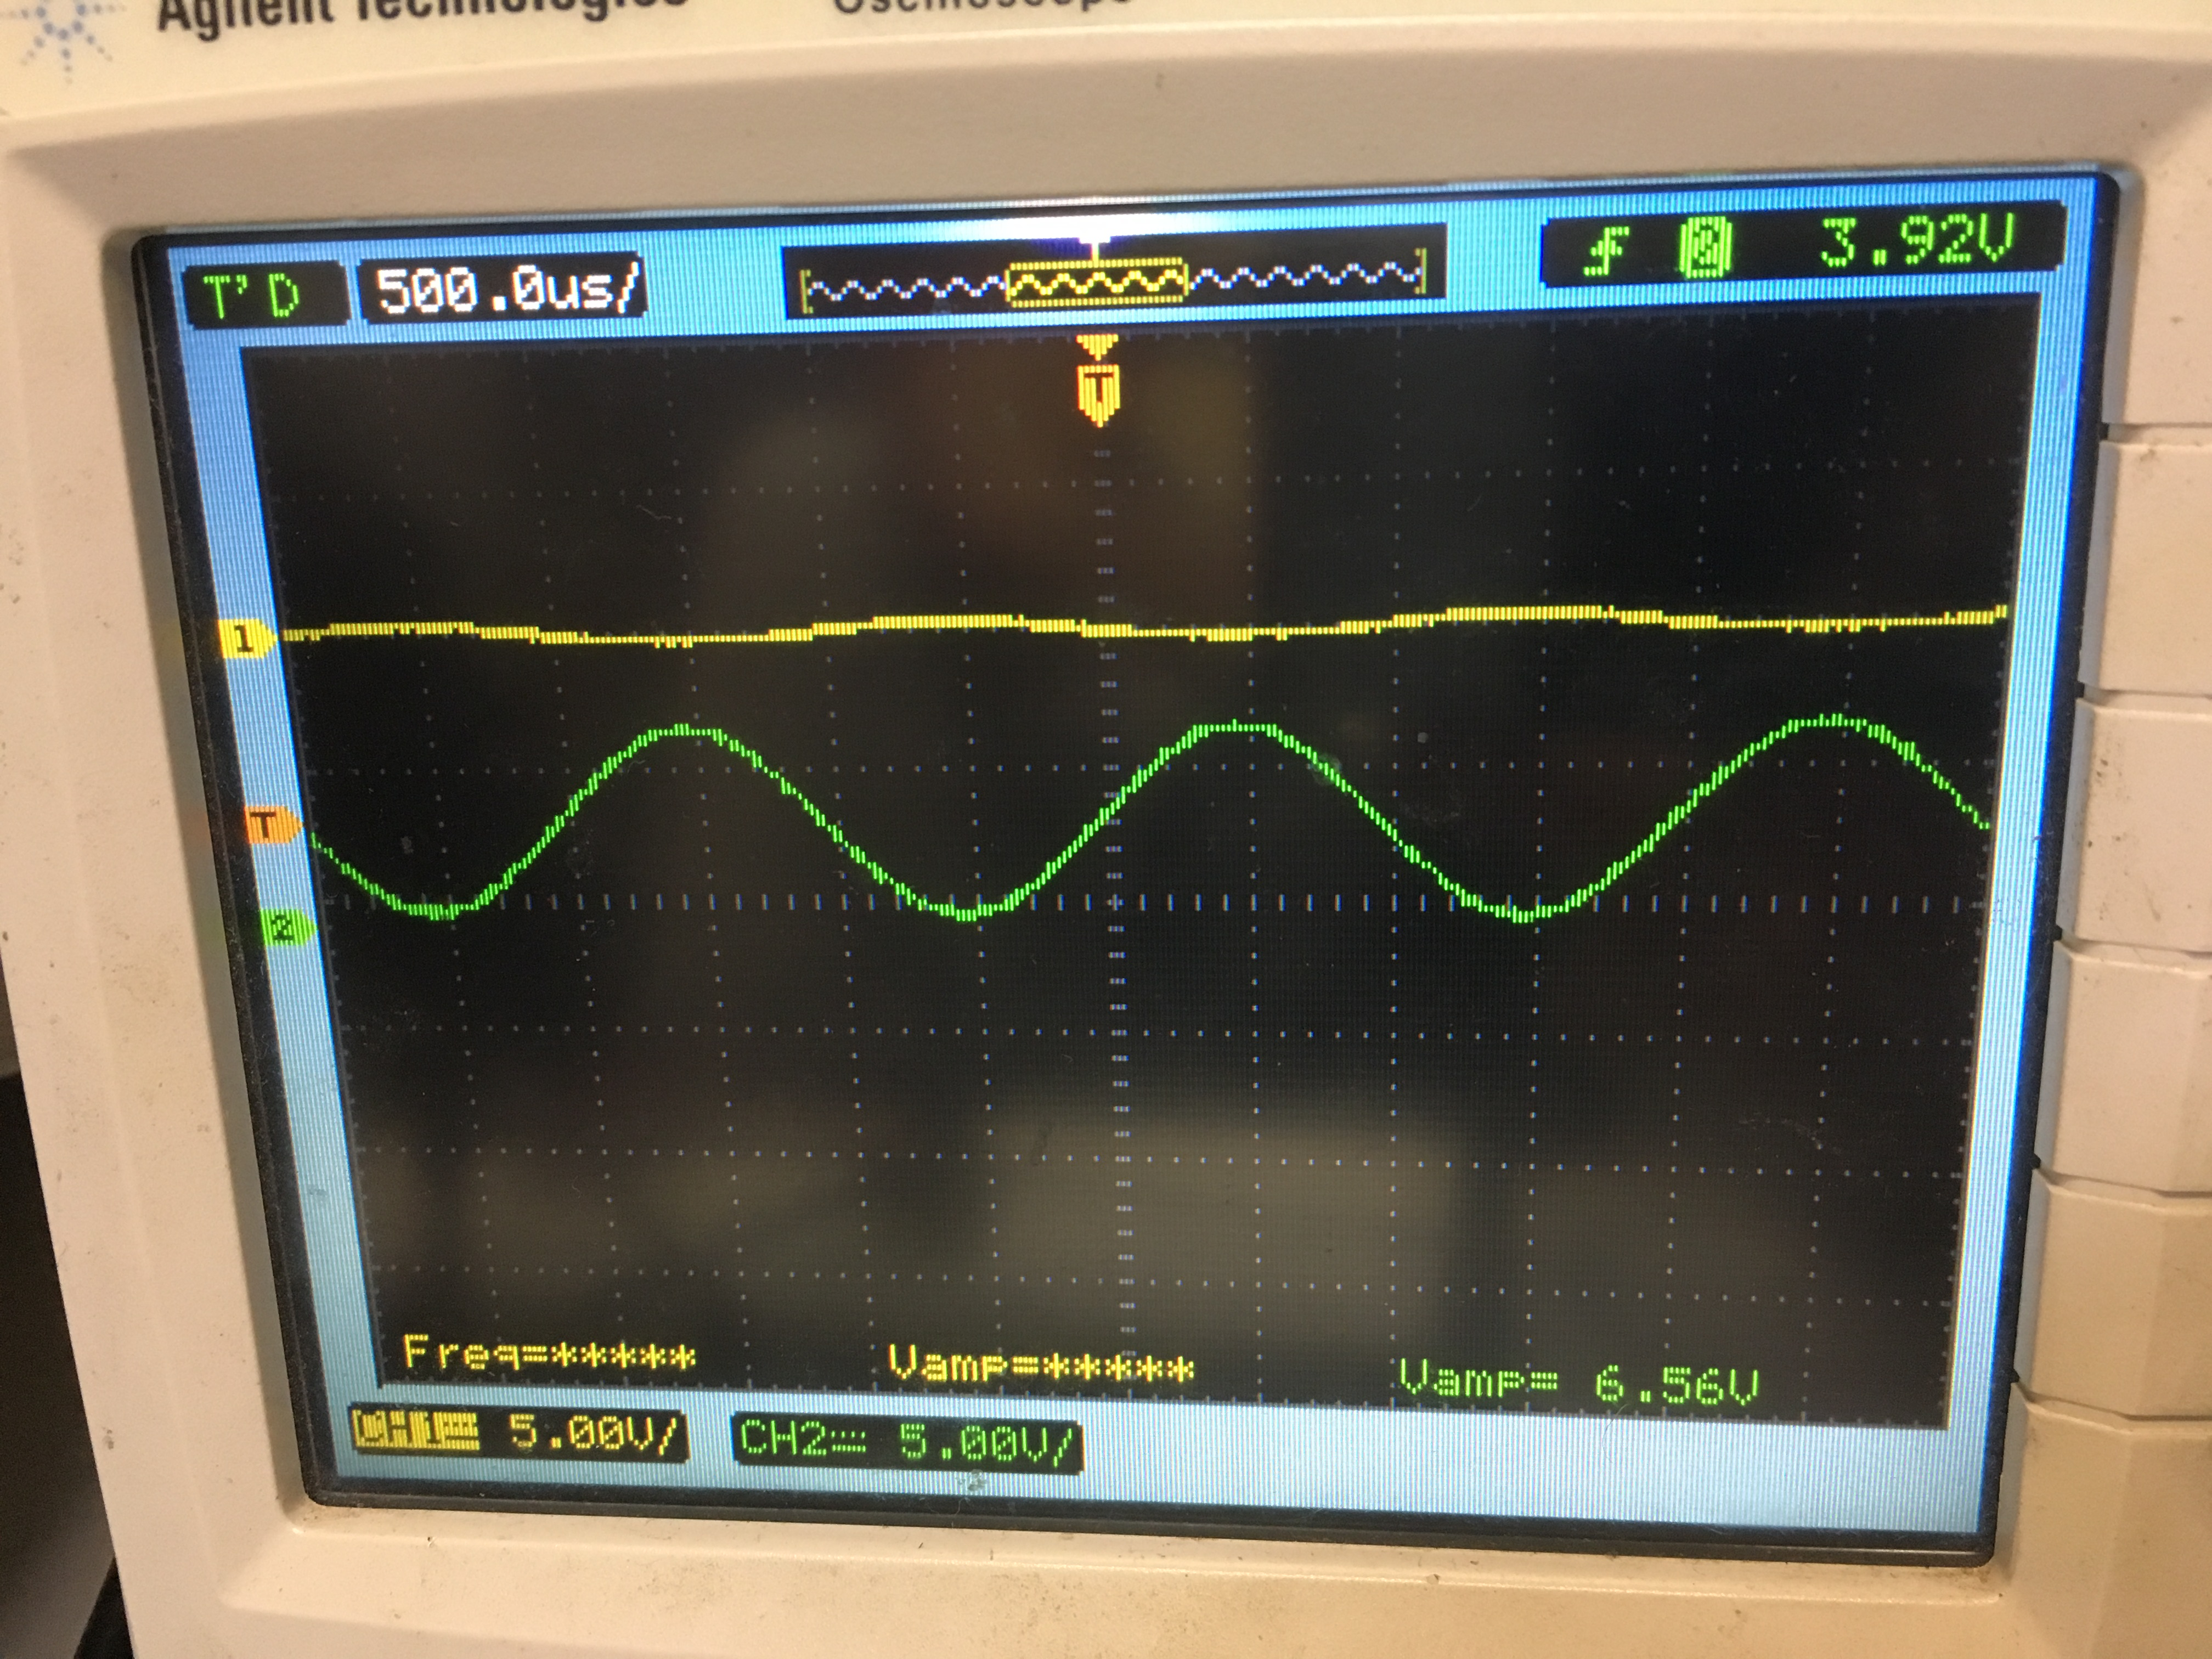
\includegraphics[height=6.5cm]{imgSource/oscilloscope/foto9.jpg}
        \caption{Sinal de saída para uma entrada com frequência de 2MHz.}
        \label{fig:foto10}
    \end{figure}

   
    %%%%%%%%%%%%%%%
    %   TABELAS   %
    %%%%%%%%%%%%%%%
    %%%%%%%%%
    % 421mV %   ====> TENSÃO DE ENTRADA NO CIRCUITO SIMULADO
    %%%%%%%%%
    \begin{table}[]
        \centering
        \begin{tabular}{|c|c|c|}
            \hline
            \rowcolor[HTML]{343434} 
            \multicolumn{1}{|l|}{\cellcolor[HTML]{343434}{\color[HTML]{EFEFEF} \textbf{Frequência (Hz)}}} & \multicolumn{1}{l|}{\cellcolor[HTML]{343434}{\color[HTML]{EFEFEF} \textbf{Vout (mV)}}} & \multicolumn{1}{l|}{\cellcolor[HTML]{343434}{\color[HTML]{EFEFEF} 
            \textbf{Ganho (dB)}}} \\ \hline
            \rowcolor[HTML]{C0C0C0} 
            {\color[HTML]{333333} 1} & {\color[HTML]{333333} 90} & {\color[HTML]{333333} 1} \\ \hline
            \rowcolor[HTML]{EFEFEF} 
            {\color[HTML]{333333} 20} & {\color[HTML]{333333} 1320} & {\color[HTML]{333333} 1} \\ \hline
            \rowcolor[HTML]{C0C0C0} 
            {\color[HTML]{333333} 100} & {\color[HTML]{333333} 1670} & {\color[HTML]{333333} 1} \\ \hline
            \rowcolor[HTML]{EFEFEF} 
            {\color[HTML]{333333} 500} & {\color[HTML]{333333} 1960} & {\color[HTML]{333333} 1} \\ \hline
            \rowcolor[HTML]{C0C0C0} 
            {\color[HTML]{333333} 1.000} & {\color[HTML]{333333} 2004} & {\color[HTML]{333333} 1} \\ \hline
            \rowcolor[HTML]{EFEFEF} 
            {\color[HTML]{333333} 5.000} & {\color[HTML]{333333} 3770} & {\color[HTML]{333333} 1} \\ \hline
            \rowcolor[HTML]{C0C0C0} 
            {\color[HTML]{333333} 10.000} & {\color[HTML]{333333} 3830} & {\color[HTML]{333333} 1} \\ \hline
            \rowcolor[HTML]{EFEFEF} 
            {\color[HTML]{333333} 20.000} & {\color[HTML]{333333} 3570} & {\color[HTML]{333333} 1} \\ \hline
            \rowcolor[HTML]{C0C0C0} 
            {\color[HTML]{333333} 50.000} & {\color[HTML]{333333} 3800} & {\color[HTML]{333333} 1} \\ \hline
            \rowcolor[HTML]{EFEFEF} 
            {\color[HTML]{333333} 100.000} & {\color[HTML]{333333} 3860} & {\color[HTML]{333333} 1} \\ \hline
            \rowcolor[HTML]{C0C0C0} 
            {\color[HTML]{333333} 500.000} & {\color[HTML]{333333} 3770} & {\color[HTML]{333333} 1} \\ \hline
            \rowcolor[HTML]{EFEFEF} 
            {\color[HTML]{333333} 1.000.000} & {\color[HTML]{333333} 3840} & {\color[HTML]{333333} 1} \\ \hline
        \end{tabular}
        \caption{Resposta em frequência do circuito para as frequências indicadas.}
        \label{table:1}
    \end{table}